\subsection{替换}

设 E 为一个 A-代数。E 上的一个拓扑称为线性拓扑，如果它在平移之下不变，并且存在一个由 E 的理想组成的 0 的基本邻域系（《一般拓扑学》，III，第223页）。此时 E 上的拓扑与其 A-代数结构相容（当 A 赋有离散拓扑时）。带线性拓扑的 A-代数称为线性拓扑化 A-代数。

命题 4. --- 设 I 是一个集合，E 是一个结合、交换、含单位元、线性拓扑化、分离且完备的 A-代数。

\begin{enumerate}
\def\labelenumi{(\roman{enumi})}
\tightlist
\item
  设 \(\varphi\) 是从 A{[}{[}I{]}{]} 到 E 中的连续同态，且 \(x_{i} = \varphi (\mathbf{X}_{i})\) 。那么：
\end{enumerate}

\begin{enumerate}
\def\labelenumi{(\alph{enumi})}
\item
  对所有 \(i \in \mathbf{I}\) ，\(x_{i}^{n}\) 当 \(n\) 趋于 \(+\infty\) 时趋于 0 ；
\item
  若 I 是无限集，则 \(x_{i}\) 沿 I 的有限子集的补集所构成的滤子趋于 0 。
\end{enumerate}

\begin{enumerate}
\def\labelenumi{(\roman{enumi})}
\setcounter{enumi}{1}
\tightlist
\item
  设 \(\mathbf{x} = (x_i)_{i\in I}\) 是 E 中满足 (i) 的条件 \(a\) 与 \(b\) 的元素族。则存在一个且仅一个保单位的连续同态 \(\varphi\) ，它从 A{[}{[}I{]}{]} 到 E 中，使得 \(\varphi (\mathbf{X}_i) = x_i\) 对所有 \(i\in I\) 。
\end{enumerate}

对所有 \(i \in I\) ，\(X_{i}^{n}\) 在 A{[}{[}I{]}{]} 中显然趋于 0 ，当 n 趋于 \(+\infty\) ；另一方面，当 I 为无限集时，\(X_{i}\) 沿 I 的有限子集的补集所构成的滤子趋于 0 。这就证明了 (i)。

设 \((x_{i})_{i\in I}\) 是 E 中满足 (i) 的条件 \(a)\) 与 \(b)\) 的元素族，设 \(\psi\) 为由 \(u\mapsto u((x_i)_{i\in I})\) 给出的、从 \(\mathbf{A}[(\mathbf{X}_i)_{i\in I}]\) 到 E 中的同态，并设 V 是 E 的 0 的一个邻域，且它是 E 的一个理想。由 \(b)\) ，存在 I 的有限子集 J 使得 \(x_{i}\in \mathbf{V}\) 对所有 \(i\in \mathrm{I - J}\) 。其次，由 \(a)\) 存在整数 \(n\geqslant 0\) 使得 \(x_{i}^{n}\in \mathbf{V}\) 对所有 \(i\in \mathrm{J}\) 。设 \(\beta\) 是 \(\mathbf{N}^{(I)}\) 中这样的元素：\(\beta_{i} = n - 1\) 对 \(i\in \mathrm{J}\) ，且 \(\beta_{i} = 0\) 对 \(i\in \mathrm{I - J}\) 。如果 \(\mathfrak{a}_{\beta}\) 表示按第 2 号开头（IV，第26页）所定义的 A{[}{[}I{]}{]} 的理想，那么

\[
u \in \mathrm{A} \left[ \left(\mathrm{X} _ {i}\right) _ {i \in I} \right] \cap \mathfrak {a} _ {\beta} \Rightarrow \psi (u) \in \mathrm{V}.
\]

这表明 \(\psi\) 是连续的，如果我们给 \(\mathbf{A}[(\mathbf{X}_i)_{i\in I}]\) 赋予由 \(\mathbf{A}[[I]]\) 的拓扑诱导的拓扑。由于 \(\mathbf{E}\) 是分离的且完备的，\(\psi\) 延拓为一个连续保单位同态 \(\varphi\) ，它从 \(\mathbf{A}[[I]]\) 到 \(\mathbf{E}\) 中。我们有 \(\varphi (\mathbf{X}_i) = \psi (\mathbf{X}_i) = x_i\) 对所有 \(i\in I\) 。最后，设 \(\varphi^{\prime}\) 是从 \(\mathbf{A}[[I]]\) 到 \(\mathbf{E}\) 中的连续保单位同态，使得 \(\varphi^{\prime}(\mathbf{X}_{i}) = x_{i}\) 。我们有 \(\varphi^{\prime}(u) = \varphi (u)\) 对所有 \(u\in \mathbf{A}[(\mathbf{X}_i)_{i\in I}]\) ，因此 \(\varphi^{\prime} = \varphi\) ，因为 \(\mathbf{A}[(\mathbf{X}_i)_{i\in I}]\) 在 \(\mathbf{A}[[I]]\) 中稠密。

我们沿用先前的记号。若 \(u \in \mathbf{A}[[\mathbf{I}]]\) ，\(u\) 在 \(\varphi\) 下的像记作 \(u(\mathbf{x})\) 或 \(u((x_i)_{i \in \mathbf{I}})\) （或亦记作 \(u(x_1, \ldots, x_n)\) ，若 \(\mathbf{I} = \{1, 2, \ldots, n\}\) ），它称为 \(\mathbf{E}\) 中以 \(x_i\) 代替 \(X_i\) 代入 \(u\) 所得的元素，或 \(u\) 当 \(x_i\) 是 \(X_i\) 的值时的值；也称为 \(u\) 当 \(X_i = x_i\) 时的值。特别地，我们有 \(u = u((X_i)_{i \in \mathbf{I}})\) 。

设 \(E'\) 是一个结合、交换、含单位元、线性拓扑化、分离且完备的 A-代数。设 \(\lambda\) 是从 E 到 \(E'\) 中的连续保单位同态，且 \((x_i)_{i \in I}\) 是 E 中满足命题 4（IV，第28页）的条件 \(a)\) 与 \(b)\) 的元素族。族 \((\lambda(x_i))_{i \in I}\) 满足同样的条件 \(a)\) 与 \(b)\) 。对每个 \(u \in A[[I]]\) 我们有

\[
\lambda \left(u \left(\left(x _ {i}\right) _ {i \in I}\right)\right) = u \left(\left(\lambda \left(x _ {i}\right)\right) _ {i \in I}\right),\tag{3}
\]

因为映射 \(u \mapsto \lambda(u((x_i)_{i \in I}))\) 是从 \(A[[I]]\) 到 \(E'\) 中的连续保单位同态，它把 \(X_i\) 变为 \(\lambda(x_i)\) 对所有 \(i \in I\) 。

如果 \(J\) 与 \(K\) 是两个集合，我们用 \(A_{J,K}\) 表示满足下列条件的所有族 \((g_j)_{j \in J}\) 构成的集合：

\begin{enumerate}
\def\labelenumi{(\roman{enumi})}
\item
  对所有 \(j \in \mathbf{J}\) ，\(g_j\) 是 \(\mathbf{A}[[\mathbf{K}]]\) 中常数项为幂零元的元素；
\item
  若 \(J\) 是无限集，则 \(g_{j}\) 沿 \(J\) 的有限子集的补集所构成的滤子趋于 0 。
\end{enumerate}

我们注意到，若 J 有限，则每个族 \((g_{j})_{j\in J}\) （由 A{[}{[}K{]}{]} 中无常数项的形式幂级数组成）都属于 \(A_{J,K}\) 。

设 \((g_j)_{j\in J}\) 属于 \(\mathbf{A}_{\mathrm{J},\mathbf{K}}\) 。由命题 3 的推论（IV，第28页），我们有 \(\lim_{n\to \infty}g_j^n = 0\) 对所有 \(j\in J\) 。设 \(f\in \mathbf{A}[[\mathrm{J}]]\) ；我们可以把 \(g_{j}\) 代入

 \(j\) 在 \(f\) 中所对应的变量，并得到一个形式幂级数 \(f((g_j)_{j \in J})\) ，它属于 A{[}{[}K{]}{]} 。此外，映射 \(f \mapsto f((g_j)_{j \in J})\) 是从 A-代数 A{[}{[}J{]}{]} 到 A{[}{[}K{]}{]} 的连续同态。

特别地，若 \(J = \{1, \ldots, p\}\) 且 \(f \in A[[X_1, \ldots, X_p]]\) ，我们可以对每个 \(X_j\) 代入一个无常数项的形式幂级数 \(g_j \in A[[K]]\) ；此代入的结果记作 \(f(g_1, \ldots, g_p)\) 。

设 \(\mathbf{x} = (x_k)_{k\in K}\) 是 E 中满足命题 4（IV，第28页）的条件 \(a\) 与 \(b\) ) 的元素族。让我们应用 (3)，取 \(\lambda\) 为由 \(u\mapsto u(\mathbf{x})\) 给出的、把 A{[}{[}K{]}{]} 映入 E 的同态；我们得到

\[
f \left(\left(g _ {j}\right) _ {j \in J}\right) (\mathbf {x}) = f \left(\left(g _ {j} (\mathbf {x})\right) _ {j \in J}\right).\tag{4}
\]

设 \(\mathbf{f} = (f_i)_{i\in I}\in (\mathbf{A}[[J]])^I\) 与 \(g = (g_j)_{j\in J}\in \mathbf{A}_{J,K}\) 。我们用 \(\mathbf{f}(\mathbf{g})\) 或 \(\mathbf{f}\circ \mathbf{g}\) 表示元素 \((f_{i}((g_{j})_{j\in J}))_{i\in I}\) ，它属于 \((\mathbf{A}[[K]])^I\) 。若 \(\mathbf{f}\in \mathbf{A}_{I,J}\) ，则 \(\mathbf{f}\circ \mathbf{g}\in \mathbf{A}_{I,K}\) ，因为映射 \(f\mapsto f((g_j)_{j\in J})\) （从 \(\mathbf{A}[[I]]\) 到 \(\mathbf{A}[[K]]\) ）是连续的。

设 \(\mathbf{f} \in (\mathbf{A}[[J]])^{\mathrm{I}}\) ，\(\mathbf{g} \in \mathbf{A}_{\mathrm{J},\mathrm{K}}\) ，\(\mathbf{h} \in \mathbf{A}_{\mathrm{K},\mathrm{L}}\) 。则 \(\mathbf{g} \circ \mathbf{h} \in \mathbf{A}_{\mathrm{J},\mathrm{L}}\) ，并且由 (4)，我们有

\[
(\mathbf {f} \circ \mathbf {g}) \circ \mathbf {h} = \mathbf {f} \circ (\mathbf {g} \circ \mathbf {h}).\tag{5}
\]

\subsection{可逆的形式幂级数}

命题 5. --- 在单个未定元的形式幂级数环 A{[}{[}T{]}{]} 中，多项式 1 - T 是可逆的，并且我们有 \((1 - \mathrm{T})^{-1} = \sum_{n=0}^{\infty} \mathrm{T}^{n}\) 。

因为

\[
(1 - \mathrm{T}) \left(\sum_ {n = 0} ^ {\infty} \mathrm{T} ^ {n}\right) = \sum_ {n = 0} ^ {\infty} \mathrm{T} ^ {n} - \sum_ {n = 0} ^ {\infty} \mathrm{T} ^ {n + 1} = 1.
\]

命题 6. --- 设 \(u \in \mathbf{A}[[\mathbf{I}]]\) ；那么，\(u\) 在 \(\mathbf{A}[[\mathbf{T}]]\) 中可逆的必要且充分条件是它的常数项在 \(\mathbf{A}\) 中可逆。

假设存在 \(v \in A[[I]]\) 使得 \(uv = 1\) 。设 \(\alpha, \beta\) 分别为 \(u\) 与 \(v\) 的常数项，则 \(\alpha\beta = 1\) ，所以 \(\alpha\) 可逆。

反之，设 \(\alpha\) 为 \(u\) 的常数项，并假设它可逆。则存在形式幂级数 \(t \in \mathbf{A}[[\mathrm{I}]]\) 使得 \(u = \alpha(1 - t)\) 且 \(\omega(t) > 0\) 。现在，存在环同态 \(\varphi: \mathbf{A}[[\mathrm{T}]] \to \mathbf{A}[[\mathrm{I}]]\) 使得 \(\varphi(\mathrm{T}) = t\) ，而 \(1 - \mathrm{T}\) 在 \(\mathbf{A}[[\mathrm{T}]]\) 中可逆（命题 5）；因之 \(1 - t\) 在 \(\mathbf{A}[[\mathrm{I}]]\) 中可逆，从而 \(u\) 也可逆。

注记. --- 设 M 为所有常数项为 1 的形式幂级数构成的集合。由命题 6，M 在乘法下构成一个交换群；A{[}{[}I{]}{]} 的乘法群因而是 M 与 A 的乘法群的直积。我们将给 M 赋予由 A{[}{[}I{]}{]} 的拓扑诱导的拓扑。对每个 \(\beta \in \mathbf{N}^{(I)}\) ，我们已在 IV 第26页定义了理想 \(a_{\beta}\) （它是 A{[}{[}I{]}{]} 的理想）；则 \(1 + a_{\beta}\) 是 M 的一个子群，且族 \((1 + a_{\beta})\) 是 M 中 1 的一个基本邻域系。由于 M 中的乘法是连续的，我们看出 M 是一个拓扑群（《一般拓扑学》，III，第223页）；换言之，映射 \(f \mapsto f^{-1}\) 在 M 中是连续的。

设 K 为一个交换域，\(\mathfrak{D}\) 为有理分式域 \(\mathrm{K}((\mathbf{X}_i)_{i\in I})\) 中由使 \(\mathbf{K}^I\) 的元素 0 可代入的有理分式组成的子环。若 \(f\in \mathfrak{D}\) ，我们有 \(f = \frac{u}{v}\) ，其中 \(u\) 与 \(v\) 是多项式，且 \(v\) 的常数项 \(\neq 0\) ，因而 \(v\) 在 \(\mathbf{K}[[\mathrm{I}]]\) 中可逆。我们可以立即验证，元素 \(uv^{-1}\) （作为 \(\mathbf{K}[[\mathrm{I}]]\) 的元素）只依赖于 \(f\) ；我们称形式幂级数 \(uv^{-1}\) 为有理分式 \(\frac{u}{v}\) 在原点的展开式。映射 \(f\mapsto uv^{-1}\) 是从 \(\mathfrak{D}\) 到 \(\mathbf{K}[[\mathrm{I}]]\) 中的单同态；我们将经常把 \(\mathfrak{D}\) 与它在此映射下的像等同。

\subsection{形式幂级数的泰勒公式}

设 \(\mathbf{X} = (\mathbf{X}_i)_{i\in I}\) 与 \(\mathbf{Y} = (\mathbf{Y}_i)_{i\in I}\) 是关于同一指标集 I 的两个未定元族。我们用 \(\mathbf{X} + \mathbf{Y}\) 表示族 \((\mathbf{X}_i + \mathbf{Y}_i)_{i\in I}\) ，它由 \(\mathbf{A}[[\mathbf{X},\mathbf{Y}]]\) 中的形式幂级数组成。显然，我们可以以 \(\mathbf{X}_i + \mathbf{Y}_i\) 代替 \(\mathbf{X}_i\) ，代入形式幂级数 \(u\in \mathbf{A}[[\mathbf{X}]]\) 中，结果记作 \(u(\mathbf{X} + \mathbf{Y})\) 。对每个 \(\nu \in \mathbf{N}^{(I)}\) ，我们用 \(\Delta^{\nu}u\) 表示 \(\mathbf{Y}^{\nu}\) 在形式幂级数 \(u(\mathbf{X} + \mathbf{Y})\) （视为属于 \(\mathbf{A}[[\mathbf{X}]][[\mathbf{Y}]]\) ）中的系数（III，第456页）。换言之，我们有

\[
u (\mathbf {X} + \mathbf {Y}) = \sum_ {\nu} \Delta^ {\nu} u (\mathbf {X}) \cdot \mathbf {Y} ^ {\nu} \quad (u \in \mathrm{A} [ [ \mathbf {X} ] ]).\tag{6}
\]

以 (0, X) 代替 (X, Y) 作代入，我们得到

\[
u (\mathbf {X}) = \sum_ {\nu} \Delta^ {\nu} u (0) \cdot \mathbf {X} ^ {\nu};\tag{7}
\]

换言之，\(\Delta^{\nu}u\) 的常数项是 \(\mathbf{X}^{\nu}\) 在 \(u\) 中的系数。由于映射 \(u \mapsto u(\mathbf{X} + \mathbf{Y})\) （从 \(\mathbf{A}[[\mathbf{X}]]\) 到 \(\mathbf{A}[[\mathbf{X}, \mathbf{Y}]]\) ）是连续的，映射 \(u \mapsto \Delta^{\nu}u\) （从 \(\mathbf{A}[[\mathbf{X}]]\) 到其自身）也是连续的。

如同多项式的情形（IV，第7页），我们可以证明公式

\begin{enumerate}
\def\labelenumi{(\arabic{enumi})}
\setcounter{enumi}{7}
\tightlist
\item
\end{enumerate}

\[
\Delta^ {\sigma} (u v) = \sum_ {\nu + \rho = \sigma} \Delta^ {\nu} (u) \Delta^ {\rho} (v),
\]

\[
\Delta^ {\rho} \Delta^ {\sigma} u = \frac {(\rho + \sigma) !}{\rho ! \sigma !} \Delta^ {\rho + \sigma} u.\tag{9}
\]

二项式公式（I，第99页，推论 2）给出 \(\Delta^{\nu}u\) 当 \(u = \sum_{\lambda} \alpha_{\lambda} X^{\lambda}\) 时的如下值

\[
\Delta^ {\nu} u = \sum_ {\lambda} \alpha_ {\lambda + \nu} \frac {(\lambda + \nu) !}{\lambda ! \nu !} X ^ {\lambda}.\tag{10}
\]

特别地考虑情形 \(\nu = \varepsilon_{i}\) ，即 \(\nu_{i} = 1\) ，\(\nu_{j} = 0\) 对 \(j \neq i\) 。我们将记 \(D_{i}u = \Delta^{\varepsilon_{i}}u\) ；换言之，\(D_{i}u\) 是 \(Y_{i}\) 在 \(u(\mathbf{X} + \mathbf{Y})\) 中的系数。于是由 (10) 我们有

\[
\mathrm{D} _ {i} u = \sum_ {\lambda} (\lambda_ {i} + 1) \alpha_ {\lambda + \varepsilon_ {i}} X ^ {\lambda};\tag{11}
\]

特别地，我们有 \(\mathbf{D}_{i}(\mathbf{X}_{i})=1\) 与 \(\mathbf{D}_{i}(\mathbf{X}_{j})=0\) 对 \(j\neq i\) 。公式 (8) 表明 \(D_{i}\) 是 A{[}{[}X{]}{]} 的一个导子，并且由 (9) 我们推出关系

\[
\mathbf {D} ^ {\nu} \boldsymbol {u} = \nu ! \Delta^ {\nu} \boldsymbol {u}\tag{12}
\]

如同多项式的情形（IV，第8页）（我们已置 \(\mathbf{D}^{\nu} = \prod_{i\in I}\mathbf{D}_{i}^{\nu_{i}}\) ，对 \(\nu = (\nu_{i})_{i\in I}\) 属于 \(\mathbf{N}^{(I)}\) ）。当 \(\mathbf{A}\) 是一个 \(\mathbf{Q}\) -代数时，公式 (6)、(7) 与 (12) 蕴含「泰勒公式」：

\begin{enumerate}
\def\labelenumi{(\arabic{enumi})}
\setcounter{enumi}{12}
\tightlist
\item
\end{enumerate}

\[
u (\mathbf {X} + \mathbf {Y}) = \sum_ {\nu} \frac {1}{\nu !} D ^ {\nu} u (\mathbf {X}). \mathbf {Y} ^ {\nu},
\]

\[
u (\mathbf {X}) = \sum_ {\nu} \frac {1}{\nu !} D ^ {\nu} u (0) \cdot X ^ {\nu}.\tag{14}
\]

注记. --- 1) 我们常说 \(D_i u\) 是 \(u\) 关于 \(X_i\) 的偏导数；我们也使用记号 \(D_{X_i} u, \frac{\partial u}{\partial X_i}\) 与 \(u_{X_i}'\) 。对单个未定元 \(X\) ，唯一的偏导数 \(Du\) （也写作 \(\frac{du}{dX}\) 或 \(u'\) ）称为 \(u\) 的导数。

\begin{enumerate}
\def\labelenumi{\arabic{enumi})}
\setcounter{enumi}{1}
\item
  公式 (9) 表明自同态 \(\Delta^{\rho}\) （即 A-模 \(\mathbf{A}[[\mathbf{X}]]\) 的自同态）两两交换。因此对自同态 \(D_i\) 而言同样成立。
\item
  如果 \(u \in \mathbf{A}[(\mathbf{X}_i)_{i \in I}]\) 是多项式，则在 IV 第6页与第7页定义的多项式 \(\Delta^{\rho} u\) 与 \(D_i u\) 跟用同样符号表示的形式幂级数一致。
\end{enumerate}

\subsection{形式幂级数代数中的导子}

设 I 为一个集合，E 为一个结合、交换、含单位元、线性拓扑化、分离且完备的 A-代数，且 \(\mathbf{x} = (x_{i})_{i \in I}\) 为 E 中满足命题 4（IV，第28页）的条件 a) 与 b) 的元素族。设 \(\varphi\) 为由 \(u \mapsto u(x)\) 给出的、把 A{[}{[}I{]}{]} 映入 E 的连续同态；它给 E 赋予一个 A{[}{[}I{]}{]}-模结构。根据 III，第552页，A{[}{[}I{]}{]} 到 A{[}{[}I{]}{]}-模 E 中的一个 A-导子 D 因而是一个 A-线性映射 D: A{[}{[}I{]}{]} → E ，满足关系

\[
\mathrm{D} (u v) = u (\mathbf {x}) \cdot \mathrm{D} (v) + \mathrm{D} (u) \cdot v (\mathbf {x})\tag{15}
\]

对 A{[}{[}I{]}{]} 中的 u, v 成立。

命题 7. --- 设 \((y_{i})_{i\in I}\) 是 E 中元素的一个族。当 I 为无限集时，我们假设 \(y_{i}\) 沿 I 的有限子集的补集所构成的滤子趋于 0 。于是存在唯一的从 A{[}{[}I{]}{]} 到 A{[}{[}I{]}{]}-模 E 中的连续 A-导子 D ，使得 \(\mathrm{D}(\mathbf{X}_{i})=y_{i}\) 对所有 \(i\in I\) 。我们有

\[
\mathrm{D} (u) = \sum_ {i \in I} (\mathrm{D} _ {i} u) (\mathbf {x}) \cdot y _ {i} \quad (u \in \mathrm{A} [ [ I ] ])  .\tag{16}
\]

由于 0 在 E 中有一个由理想组成的基本邻域系，族 \(((\mathrm{D}_i u)(\mathbf{x}) \cdot y_i)_{i \in I}\) 在 E 中可和，对所有 \(u \in A[[I]]\) （《一般拓扑学》，III，第263页，推论 2）。于是公式 (16) 定义了一个 A-线性映射 \(\mathbf{D}: A[[I]] \to E\) 。我们留给读者验证 D 是一个连续导子。设 \(\mathbf{D}_1\) 是从 A{[}{[}I{]}{]} 到 E 中的一个连续 A-导子，使得 \(\mathbf{D}_1(\mathbf{X}_i) = y_i\) 对所有 \(i \in I\) 。连续导子 \(\mathbf{D} - \mathbf{D}_1\) 的核是 A{[}{[}I{]}{]} 的一个包含 1 与诸未定元 \(X_{i}\) 的闭子代数 B。由于多项式代数 \(\mathbf{A}[(\mathbf{X}_{i})_{i\in I}]\) 在 A{[}{[}I{]}{]} 中稠密，我们有 \(B = A[[I]]\) ，从而 \(D_{1} = D\) 。

推论 1. --- 设 \(\Delta\) 为 A-代数 E 的一个连续导子。对每个形式幂级数 \(u \in \mathbf{A}[[\mathrm{I}]]\) ，族 \(((\mathrm{D}_i u)(\mathbf{x}) \cdot \Delta x_i)_{i \in I}\) 可和，并且我们有

\[
\Delta (u (\mathbf {x})) = \sum_ {i \in I} \left(\mathrm{D} _ {i} u\right) (\mathbf {x}) \cdot \Delta x _ {i}.\tag{17}
\]

这由命题 7 得出，因为映射 \(u \mapsto \Delta(u(\mathbf{x}))\) 是从 \(\mathbf{A}[[\mathbf{I}]]\) 到 \(\mathbf{A}[[\mathbf{I}]]\) -模 \(\mathbf{E}\) 中的一个连续导子。

推论 2. --- 导子 \(D_{i}\) 是 A-代数 A{[}{[}I{]}{]} 的唯一连续导子，使得

\[
\mathrm{D} _ {i} (\mathrm{X} _ {i}) = 1, \quad \mathrm{D} _ {i} (\mathrm{X} _ {j}) = 0 \quad f o r \quad j \neq i.\tag{18}
\]

这由推论 1 得出。

推论 3. --- 设 \(f \in \mathbf{A}[[\mathbf{X}_1, \ldots, \mathbf{X}_p]]\) 与 \(g_i \in \mathbf{A}[[\mathbf{Y}_1, \ldots, \mathbf{Y}_q]]\) ，对 \(1 \leqslant i \leqslant p\) 。假设对 \(1 \leqslant i \leqslant p\) ，\(g_i\) 的常数项为零，并令 \(h = f(g_1, \ldots, g_p)\) 。则对 \(1 \leqslant j \leqslant q\) 我们有

\[
\frac {\partial h}{\partial \mathbf {Y} _ {j}} = \sum_ {i = 1} ^ {p} \mathrm{D} _ {i} f (g _ {1}, \dots , g _ {p}) \cdot \frac {\partial g _ {i}}{\partial \mathbf {Y} _ {j}}.\tag{19}
\]

这是推论 1 的特殊情形：\(\mathbf{E} = \mathbf{A}[[\mathbf{Y}_1,\dots ,\mathbf{Y}_q]]\) ，\(x_{i} = q_{i}\) 且 \(\Delta = \partial /\partial \mathbf{Y}_j\) 。

命题 8. --- 设 \(\mathbf{X} = (\mathbf{X}_i)_{i\in I}\) 是由有限个未定元组成的族。

\begin{enumerate}
\def\labelenumi{(\roman{enumi})}
\item
  形式幂级数环 A{[}{[}X{]}{]} 的每个导子都是连续的。
\item
  从多项式环 A{[}X{]} 到形式幂级数环 A{[}{[}X{]}{]} 中的每个导子都以唯一的方式延拓为环 A{[}{[}X{]}{]} 的导子。
\item
  族 \((\mathbf{D}_i)_{i\in I}\) 是 \(\mathbf{A}[[\mathbf{X}]]\) -模的一组基，该模由 \(\mathbf{A}\) -导子（把 \(\mathbf{A}[[\mathbf{X}]]\) 映入其自身）组成。
\end{enumerate}

设 \(\mathfrak{b}_n\) 为所有阶 \(\geqslant n\) 的形式幂级数组成的集合。显然 \(\mathfrak{b}_n\) 是环 \(A[[X]]\) 中的理想，由 \(n\) 次单项式生成。因此 \(\mathfrak{b}_n\) 由 \(n\) 个无常数项的形式幂级数之积的有限和组成；如果 \(D\) 是 \(A[[X]]\) 的一个导子，则我们有

\[
\mathrm{D} (f _ {1} \dots f _ {n}) = \sum_ {i = 1} ^ {n} f _ {1} \dots f _ {i - 1} \mathrm{D} (f _ {i}) f _ {i + 1} \dots f _ {n},
\]

由此立即得出 \(\mathbf{Db}_{n} \subset \mathbf{b}_{n-1}\) 对 \(n \geqslant 1\) 。由于序列 \((\mathfrak{b}_n)_{n \geqslant 0}\) 是 A{[}{[}X{]}{]} 中 0 的一个基本邻域系（IV，第26页注记），D 是连续的，(i) 得证。

设 \(\Delta\) 是从 A{[}X{]} 到 A{[}{[}X{]}{]} 中的一个导子。如前面那样论证，我们可以证明 \(\Delta(h)\) 属于 \(\mathfrak{b}_{n-1}\) ，对每个齐次多项式 \(h\) （次数 \(n \geqslant 1\) ）。现在设 \(u \in \mathbf{A}[[\mathbf{X}]]\) ，并设 \(u_n\) 是其次数为 \(n\) 的齐次分量，取自 \(u\) 。由于 \(\Delta(u_n) \in \mathfrak{b}_{n-1}\) 对 \(n \geqslant 1\) ，族 \((\Delta(u_n))_{n \geqslant 0}\) 在 A{[}{[}X{]}{]} 中可和，从而我们可以定义 A{[}{[}X{]}{]} 到其自身的一个导子 D ，通过

\[
\mathrm{D} (u) = \sum_ {n \geqslant 0} \Delta \left(u _ {n}\right).
\]

我们有 \(D(\mathfrak{b}_n) \subset \mathfrak{b}_{n-1}\) ，因此 \(D\) 是 \(A[[X]]\) 的加法群的一个连续自同态。映射 \(\Phi: (u, v) \mapsto D(uv) - uD(v) - D(u)v\) （从 \(A[[X]] \times A[[X]]\) 到 \(A[[X]]\) ）是连续的，且在 \(A[X] \times A[X]\) 上为零。由于 \(A[X]\) 在 \(A[[X]]\) 中稠密，我们有 \(\Phi = 0\) ；换言之，\(D\) 是 \(A[[X]]\) 到其自身的一个导子，并且是 \(\Delta\) 的延拓。

最后，A{[}X{]} 在 A{[}{[}X{]}{]} 中稠密，且 A{[}{[}X{]}{]} 的每个导子由 (i) 知是连续的；因此存在 \(\Delta\) 到 A{[}{[}X{]}{]} 的导子的唯一延拓。这就证明了 (ii)。

仍需证明 (iii)。公式 (18)（IV，第33页）表明族 \((\mathbf{D}_i)_{i\in I}\) 在 \(\mathbf{A}[[\mathbf{X}]]\) 上线性无关，而公式 (16)（IV，第32页）应用于 \(\mathbf{E} = \mathbf{A}[[\mathbf{X}]]\) 的情形，表明每个 A-导子都是诸 \(\mathbf{D}_i\) 的、系数在 \(\mathbf{A}[[\mathbf{X}]]\) 中的线性组合。

命题 9. --- 设 \((u_{\lambda})_{\lambda \in L}\) 是 A{[}{[}I{]}{]} 中元素的一个无常数项的可和族，D 是 A-代数 A{[}{[}I{]}{]} 的一个连续导子。若 \(f = \prod_{\lambda \in L} (1 + u_{\lambda})\) （IV，第27页，命题 2），则族 \((D u_{\lambda} / (1 + u_{\lambda}))_{\lambda \in L}\) 是

可求和且我们有

\[
\mathrm{D} (f) / f = \sum_ {\lambda \in L} \mathrm{D} (u _ {\lambda}) / (1 + u _ {\lambda}).\tag{20}
\]

如果 \(g\) 与 \(h\) 是 \(\mathbf{A}[[\mathbf{I}]]\) 的两个可逆元素，则

\[
\mathrm{D} (g h) = h. \mathrm{D} g + g. \mathrm{D} h
\]

因此，除以gh后，

\[
\mathrm{D} (g h) / g h = \mathrm{D} (g) / g + \mathrm{D} (h) / h.\tag{21}
\]

对 L 的每个有限子集 M，令 \(f_{M} = \prod_{\lambda \in M} (1 + u_{\lambda})\) 。由 (21)，我们对 Card M 作归纳推出关系

\[
\mathrm{D} \left(f _ {\mathrm{M}}\right) / f _ {\mathrm{M}} = \sum_ {\lambda \in \mathrm{M}} \mathrm{D} \left(u _ {\lambda}\right) / \left(1 + u _ {\lambda}\right).\tag{22}
\]

这证明了当 L 有限时命题 9 成立。现在假设 L 无限，并用 F 表示 L 的有限子集构成的滤过有序集。我们有 \(\lim_{\mathfrak{F}} f_{M} = f\) ，因此（IV，第30页，注记）

\[
\mathrm{D} (f) / f = \lim _ {\mathfrak {F}} \mathrm{D} (f _ {\mathrm{M}}) / f _ {\mathrm{M}}.
\]

于是命题 9 由对 (22) 取极限得出。

\subsection{形式幂级数环中方程的解}

引理 2. --- 设 \((g_i)_{i \in I}\) 是一族阶 \(\geqslant 2\) 的元素，位于 A{[}{[}I{]}{]} 中。当 I 为无限时，假设 \(g_i\) 沿 I 的有限子集的补集构成的滤子趋于 0 。存在且仅存在拓扑 A-代数 A{[}{[}I{]}{]} 的一个自同构 T ，使得对所有 i ∈ I，有 T(X \(_i\) ) = X \(_i\) + g \(_i\) 。进一步，

\[
\omega (\mathrm{T} (u) - u) \geqslant \omega (u) + 1\tag{23}
\]

对 \(u \in \mathbf{A}[[\mathrm{I}]]\) 成立。

级数 \(f_{i} = \mathbf{X}_{i} + g_{i}\) 没有常数项，且当 I 无限时 \(f_{i}\) 沿 I 的有限子集的补集构成的滤子趋于 0 。因此（IV，第28页，命题 4）存在恰好一个 A-代数 A{[}{[}I{]}{]} 的连续自同态 T ，使得 \(\mathrm{T}(\mathbf{X}_i) = f_i\) 对所有 \(i \in I\) 。对每个 \(\nu \in \mathbf{N}^{(I)}\) 我们令

\[
v _ {\nu} = \mathrm{T} \left(\mathbf {X} ^ {\nu}\right) - \mathbf {X} ^ {\nu} = \prod_ {i \in I} \left(\mathbf {X} _ {i} + g _ {i}\right) ^ {\nu (i)} - \prod_ {i \in I} \mathbf {X} _ {i} ^ {\nu (i)};
\]

关系 \(\omega(g_i) \geqslant 2\) 蕴含 \(\omega(v_\nu) \geqslant |\nu| + 1\) ，并且关系式 (23) 由此立即得出。

让我们证明 T 是单射。给定 \(u \in A[[I]]\) 使得 \(T(u) = 0\) ，由 (23) 我们有 \(\omega(u) \geqslant \omega(u) + 1\) ，如果 \(u \neq 0\) 则这是不可能的，因为 \(\omega(u)\) 将是一个正整数。

对每个形式级数 \(v\) （位于 \(A[[I]]\) 中），我们用 \(H_n(v)\) 表示它的 \(n\) 次齐次分量。令 \(S_0(v) = H_0(v)\) ，并用递推方程定义连续映射 \(S_n: A[[I]] \to A[[I]]\)

\[
\mathrm{S} _ {n} (v) = \mathrm{H} _ {n} \left(v - \mathrm{T} \left(\sum_ {k = 0} ^ {n - 1} \mathrm{S} _ {k} (v)\right)\right) \quad \text { for } \quad n \geqslant 1.\tag{24}
\]

令 \(S(v) = \sum_{n \geqslant 0} S_n(v)\) ；如果 \(\nu \in \mathbf{N}^{(I)}\) 且 \(n = |\nu|\) ，则系数 \(S^{\nu}(v)\) ，即

\(X^{\nu}\) 在 \(S(v)\) 中的系数，等于 \(X^{\nu}\) 在 \(S_{n}(v)\) 中的系数；由于 \(S_{n}\) 是连续映射，映射 \(S^{\nu}: A[[I]] \to A\) 是连续的。因此，根据 \(A[[I]] = A^{N^{(I)}}\) 上乘积拓扑的定义，映射 \(S: A[[I]] \to A[[I]]\) 是连续的。

我们将证明关系式 \(\mathrm{T}(\mathrm{S}(v)) = v\) 对所有 \(v \in A[[I]]\) 成立，这将完成引理的证明。设 \(v \in A[[I]]\) ，\(u_n = S_n(v)\) 且 \(u = S(v)\) 。设 n 为正整数，使得

\[
\omega (v - \mathrm{T} (u)) \geqslant n.\tag{$(25)_{n}$}
\]

我们有 \(\omega(u - (u_{0} + \cdots + u_{n-1})) \geqslant n\) ，从而

\[
\omega (\mathrm{T} (u) - \mathrm{T} (u _ {0} + \dots + u _ {n - 1}) - u _ {n}) \geqslant n + 1\tag{26}
\]

由 (23)，现在递推方程 (24) 表明

\[
u _ {n} = \mathrm{H} _ {n} (v - \mathrm{T} (u _ {0} + \dots + u _ {n - 1}))\tag{27}
\]

由 (26)，形式幂级数 \(v - \mathrm{T}(u)\) 与 \(v - \mathrm{T}(u_{0} + \cdots + u_{n-1}) - u_{n}\) 有相同的 n 次齐次分量，且由 (27) 该分量为零。于是我们有 \(\omega(v - \mathrm{T}(u)) \geqslant n + 1\) ，即 \((25)_{n}\) 蕴含 \((25)_{n+1}\) 。由于 \((25)_{0}\) 显然成立，我们遂有 \(\omega(v - \mathrm{T}(u)) \geqslant n\) 对每个整数 \(n \geqslant 0\) ，从而 \(v = \mathrm{T}(u) = \mathrm{T}(\mathrm{S}(v))\) ，此即所要证明的。

在本节其余部分中，对于任意集合 I，我们将用 A \{I\} 表示满足以下条件的族 \((f_i)_{i\in I}\) 的集合：

\begin{enumerate}
\def\labelenumi{(\roman{enumi})}
\item
  对每个 \(i \in I\) ，\(f_i\) 是 A{[}{[}I{]}{]} 的一个无常数项的元素；
\item
  若 I 是无限的，则 \(f_{i}\) 沿 I 的有限子集的补集所构成的滤子趋于 0。
\end{enumerate}

集合 A\{I\} 对复合律 \((\mathbf{f},\mathbf{g})\mapsto\mathbf{f}\circ\mathbf{g}\) 成一个幺半群，以 \(\{X_{i}\}_{i\in I}\) 为单位元。因此 A\{I\} 的可逆元素之集是一个群。

另一方面，设 E 为 A-代数 \(\mathbf{A}[[\mathrm{I}]]\) 的所有保持无常数项形式幂级数组成的理想不变的连续保单位自同态构成的幺半群。如果 \(\mathbf{f} \in \mathbf{A}\{\mathbf{I}\}\) 且 \(g \in \mathbf{A}[[\mathrm{I}]]\) ，则元素 \(g(\mathbf{f})\) 有定义。对固定的 \(\mathbf{f}\) ，映射 \(g \mapsto g(\mathbf{f})\) （从 \(\mathbf{A}[[\mathrm{I}]]\) 到其自身）是 E 的一个元素 \(\mathbf{W}_{\mathbf{f}}\) 。如果 \(\mathbf{f}_1, \mathbf{f}_2 \in \mathbf{A}\{\mathbf{I}\}\) 且 \(g \in \mathbf{A}[[\mathrm{I}]]\) ，由公式 (5)（IV，第30页）我们有

\[
\mathbf {W} _ {\mathbf {f} _ {1} \circ \mathbf {f} _ {2}} (g) = g (\mathbf {f} _ {1} \circ \mathbf {f} _ {2}) = g (\mathbf {f} _ {1}) \circ \mathbf {f} _ {2} = \mathbf {W} _ {\mathbf {f} _ {2}} (\mathbf {W} _ {\mathbf {f} _ {1}} (g))
\]

因此 \(\mathbf{f} \mapsto \mathbf{W}_{\mathbf{f}}\) 是从与 A \{I\} 相反的幺半群到 E 中的一个同态。由命题 4（IV，第28页），此同态是双射的。

设 \(\mathbf{f} = (f_i)_{i\in I}\in \mathbf{A}\{\mathbf{I}\}\) ，并令 \(\sum_{j\in I}\alpha_{ij}\mathbf{X}_j\) 为

\(f_{i}\) 的 1 次齐次分量。对 I 中任意固定的 \(j\) ，我们有 \(\alpha_{ij} = 0\) ，除有限个下标 \(i\) 外，这由上述假设 (ii) 可知。若 \((\lambda_i) \in \mathbf{A}^{(I)}\) ，我们遂有 \(\left(\sum_{j \in I} \alpha_{ij} \lambda_j\right) \in \mathbf{A}^{(I)}\) 。

我们用 \(T_{f}\) 表示 A-线性映射 \(^{1}\)

\[
\left(\lambda_ {i}\right) \mapsto \left(\sum_ {j \in I} \alpha_ {i j} \lambda_ {j}\right)
\]

（从 \(\mathbf{A}^{(I)}\) 到 \(\mathbf{A}^{(I)}\) ）。若 \(\mathbf{g} \in \mathbf{A}\{I\}\) ，则容易验证

\[
\mathrm{T} _ {\mathbf {f} \circ \mathbf {g}} = \mathrm{T} _ {\mathbf {f}} \circ \mathrm{T} _ {\mathbf {g}}.\tag{28}
\]

命题 10. --- 设 \(\mathbf{f} \in \mathbf{A}\{\mathbf{I}\}\) ；则下列条件等价：(i) \(\mathbf{f}\) 在 \(\mathbf{A}\{\mathbf{I}\}\) 中对运算 \(\circ\) 可逆；

\begin{enumerate}
\def\labelenumi{(\roman{enumi})}
\setcounter{enumi}{1}
\tightlist
\item
  \(\mathbf{T}_{\mathbf{f}}\) 在环 \(\operatorname{End}(\mathbf{A}^{(I)})\) 中可逆。
\end{enumerate}

中可逆。蕴含关系 (i) \(\Rightarrow\) (ii) 由 (28) 直接得出。现在设 \(T_{f}\) 在 \(\operatorname{End}(A^{(I)})\) 中可逆。存在 \(\mathbf{g} = (g_i)_{i \in I} \in A\{I\}\) ，使得每个 \(g_i\) 都是 1 次齐次的，且 \(T_{g} \circ T_{f}\) 是 \(A^{(I)}\) 的恒等映射。记 \(\mathbf{h} = \mathbf{g} \circ \mathbf{f}\) ；则 (28) 表明 \(T_{h}\) 是 \(A^{(I)}\) 的恒等映射，这等价于断言 \(\omega(h_i - X_i) \geqslant 2\) 。由 IV 第35页的引理 2，h 因此在 A \{I\} 中可逆。显然 \(\mathbf{g}\) 在 A \{I\} 中可逆，因此 \(\mathbf{f}\) 在 A \{I\} 中可逆。

推论. --- 设 \(f_{i}(Y_{1}, Y_{2}, \ldots, Y_{q}, X_{1}, X_{2}, \ldots, X_{p}) (1 \leqslant i \leqslant q)\) 是 A{[}{[} \(Y_{1}, \ldots, Y_{q}, X_{1}, \ldots, X_{p}\) {]}{]} 中 q 个无常数项的形式幂级数。若形式幂级数 D = det \(\left(\frac{\partial f_{i}}{\partial Y_{j}}\right)\) 的常数项在 A 中可逆，则存在恰好一组 q 个形式幂级数 \(u_{1}(X_{1}, \ldots, X_{p}), \ldots, u_{q}(X_{1}, \ldots, X_{p})\) ，使得

\[
f _ {i} (u _ {1}, \dots , u _ {q}, \mathrm{X} _ {1}, \dots , \mathrm{X} _ {p}) = 0 \quad (1 \leqslant i \leqslant q).\tag{29}
\]

令 \(f_{q+1} = \mathbf{X}_1, \ldots, f_{q+p} = \mathbf{X}_p\) ，\(\mathbf{f} = (f_1, \ldots, f_{p+q})\) ，则 \(\det \mathbf{T}_{\mathbf{f}}\) 等于 \(\mathbf{D}\) 的常数项，从而在 \(\mathbf{A}\) 中可逆；于是 \(\mathbf{T}_{\mathbf{f}}\) 可逆。由命题 10，存在无常数项的形式幂级数

\[
\boldsymbol {g} _ {1}, \dots , \boldsymbol {g} _ {q + p} \in \mathrm{A} \left[ \left[ \mathrm{Y} _ {1}, \dots , \mathrm{Y} _ {q}, \mathrm{X} _ {1}, \dots , \mathrm{X} _ {p} \right] \right]
\]

使得当记

\[
\mathbf {g} = \left(g _ {1}, \dots , g _ {p + q}\right), \quad \mathbf {1} _ {p + q} = \left(\mathrm{Y} _ {1}, \dots , \mathrm{Y} _ {q}, \mathrm{X} _ {1}, \dots , \mathrm{X} _ {p}\right)
\]

时，我们有 \(\mathbf{f} \circ \mathbf{g} = \mathbf{g} \circ \mathbf{f} = \mathbf{1}_{p + q}\) 。关系式 \(\mathbf{f} \circ \mathbf{g} = \mathbf{1}_{p + q}\) 特别地给出

\[
\boldsymbol {g} _ {q + 1} = \mathbf {X} _ {1}, \dots , \boldsymbol {g} _ {q + p} = \mathbf {X} _ {p}.
\]

因此

\[
f _ {i} \left(g _ {1}, \dots , g _ {q}, \mathrm{X} _ {1}, \dots , \mathrm{X} _ {p}\right) = \mathrm{Y} _ {i} \quad (1 \leqslant i \leqslant q).\tag{30}
\]

现在令

\[
u _ {i} \left(\mathrm{X} _ {1}, \dots , \mathrm{X} _ {p}\right) = g _ {i} (0, \dots , 0, \mathrm{X} _ {1}, \dots , \mathrm{X} _ {p}) \quad (1 \leqslant i \leqslant q);\tag{31}
\]

以 0 代替每个 \(\mathbf{Y}_i\) 代入 (30) ，我们得到所要的关系式 (29)。

反之，假设形式幂级数 \(u_1, \ldots, u_q\) （属于环 \(A[[X_1, \ldots, X_p]]\) ）满足关系式 (29)。关系式 \(\mathbf{g} \circ \mathbf{f} = 1_{p + q}\) 蕴含

\[
g _ {i} (f _ {1}, \dots , f _ {q}, \mathrm{X} _ {1}, \dots , \mathrm{X} _ {p}) = \mathrm{Y} _ {i} \quad (1 \leqslant i \leqslant q);\tag{32}
\]

并在 (32) 中以 \(u_{i}\) 代 \(Y_{i}\) （对 \(1 \leqslant i \leqslant q\) ），我们得到 (31)，由此得出方程组 (29) 的解的唯一性。

\subsection{整环上的形式幂级数}

命题 11. --- 假设 A 是一个整环。

\begin{enumerate}
\def\labelenumi{(\roman{enumi})}
\item
  环 A{[}{[}I{]}{]} 仍是一个整环。
\item
  如果 \(u, v\) 是 \(\mathbf{A}[[\mathbf{I}]]\) 的非零元素，则 \(\omega(uv) = \omega(u) + \omega(v)\) 。
\end{enumerate}

对每个 \(J \subset I\) ，令 \(\varphi_{J}\) 为从 A{[}{[}I{]}{]} 到 A{[}{[}J{]}{]} 的同态，它是在 A{[}{[}I{]}{]} 的每个元素中以 \(X_{i}\) 代 \(X_{i}\) （当 \(i \in J\) ）并以 0 代 \(X_{i}\) （当 \(i \in I - J\) ）而得到的。设 u, v 为 A{[}{[}I{]}{]} 的非零元素，\(p = \omega(u)\) ，\(q = \omega(v)\) ；存在 I 的一个有限子集 J，使得

\[
\varphi_ {J} (u) \neq 0, \quad \varphi_ {J} (v) \neq 0, \quad \omega (\varphi_ {J} (u)) = p, \quad \omega (\varphi_ {J} (v)) = q.
\]

设 \(a\) （相应地 \(b\) ）是次数为 \(p\) （相应地 \(q\) ）的齐次分量，取自 \(\varphi_{J}(u)\) （相应地 \(\varphi_{J}(v)\) ）。由于 \(J\) 有限，\(a\) 与 \(b\) 是多项式。我们有 \(a \neq 0\) ，\(b \neq 0\) ，因此 \(ab \neq 0\) （IV，第9页，命题 8）。于是 \(\varphi_{J}(u) \varphi_{J}(v)\) 非零，且阶为 \(p + q\) 。由此可知 \(uv \neq 0\) 且 \(\omega(uv) \leqslant p + q\) ；但显然 \(\omega(uv) \geqslant p + q\) 。

\subsection{一个域上的一元形式幂级数环的分式域}

若 K 是一个交换域，我们将用 \(\mathrm{K}((\mathbf{X}))\) 表示整环 \(\mathrm{K}[[\mathbf{X}]]\) 的分式域。

命题 12. --- K((X)) 的每个非零元素 u 都可以唯一地写成 \(u = X^{k}v\) ，其中 \(k \in Z\) 且 v 是 X 的 0 阶形式幂级数。设 u = w/t，其中 w, t 是 K{[}{[}X{]}{]} 的非零元素。我们有 \(w = X^{r}w_{1}, t = X^{s}t_{1}\) ，其中 r, \(s \in N\) 且 \(w_{1}, t_{1}\) 是 0 阶形式幂级数，从而在 K{[}{[}X{]}{]} 中可逆（IV，第30页，命题 6）。于是 \(u = X^{r-s}w_{1}t_{1}^{-1}\) ，且 \(w_{1}t_{1}^{-1}\) 是 0 阶形式幂级数。

我们来证明唯一性。假设 \(u = X^{k_{1}}v_{1} = X^{k_{2}}v_{2}\) ，其中 \(k_{1}, k_{2} \in Z\) 且 \(v_{1}, v_{2}\) 是 0 阶形式幂级数。由于 \(X^{k_{1}-k_{2}} = v_{2}v_{1}^{-1}\) 是 0 阶形式幂级数，我们有 \(k_{1} = k_{2}\) ，由此 \(v_{1} = v_{2}\) ，这就证明了唯一性断言。

我们将称 \(\mathbf{K}((\mathbf{X}))\) 中的元素为 X 中系数在 K 内的广义形式幂级数，或者在没有混淆时简称为形式幂级数（ \(K[[X]]\) 中的元素则称为具有正指数的形式幂级数）；若 \(u \neq 0\) ，命题 12 中定义的整数 k 也称为 u 的阶，并记作 \(\omega(u)\) ，即使它是 \textless{} 0 时也如此；我们还记 \(\omega(0) = \infty\) 。可以立即验证

\[
\begin{array}{l} \omega (u + v) \geqslant \inf (\omega (u), \omega (v)) \\ \omega (u + v) = \inf (\omega (u), \omega (v)) \quad \text { if } \quad \omega (u) \neq \omega (v) \\ \omega (u v) = \omega (u) + \omega (v) \end{array}
\]

对广义形式幂级数仍然成立。特别地，若 \(u \neq 0\) ，则 \(\omega(u^{-1}) = -\omega(u)\) 。* 换言之（《交换代数》，VI，第 3 节，第 6 号，第 392 页，定义 3），\(\omega\) 是域 \(K((X))\) 的一个规范化离散赋值。*

对每个整数 \(n \in \mathbf{Z}\) ，令 \(\mathfrak{p}_n\) 为所有 \(u \in K((X))\) （其中 \(\omega(u) \geqslant n\) ）组成的集合。则 \((\mathfrak{p}_n)_{n \in \mathbf{Z}}\) 是加法群 \(K((X))\) 的一个递减子群序列，其交为 0；因此在 \(K((X))\) 上存在一个在平移下不变的拓扑，使得 \((\mathfrak{p}_n)_{n \in \mathbf{Z}}\) 是 0 的基本邻域系（《一般拓扑学》，III，第223页）。我们容易验证 \(K((X))\) 是一个拓扑域（《一般拓扑学》，III，第281页），并且 \(K[[X]]\) 是 \(K((X))\) 的开且闭子空间。

设 \((\alpha_{n})_{n\in \mathbf{Z}}\) 是 \(\mathbf{K}\) 中元素的一个族，并假设存在整数 \(\mathbf{N}\) 使得 \(\alpha_{n} = 0\) 对所有 \(n < \mathbf{N}\) 。则族 \((\alpha_{n}\mathbf{X}^{n})_{n\in \mathbf{Z}}\) 在 \(\mathbf{K}((\mathbf{X}))\) 中可和（《一般拓扑学》，III，第263页，推论）；令 \(u = \sum_{n\in \mathbf{Z}}\alpha_n\mathbf{X}^n\) ，则 \(u = 0\) 当且

仅当 \(\alpha_{n} = 0\) 对所有 \(n\) ；否则 \(u\) 的阶是最小整数 \(k\) ，它使 \(\alpha_{k} \neq 0\) 。最后，\(\mathbf{K}((\mathbf{X}))\) 的每个元素都可以唯一地写成 \(\sum_{n \in \mathbf{Z}} \alpha_{n} \mathbf{X}^{n}\) 的形式，其中序列 \((\alpha_{n})\) 满足 \(\alpha_{-n} = 0\) 对所有充分大的 \(n\) 。

由于环 K{[}X{]} 是 K{[}{[}X{]}{]} 的子环，每个有理分式 \(u/v \in \mathrm{K}(\mathrm{X})\) （u, v 为 X 的多项式）都可以等同于 K((X)) 中的（广义）形式幂级数 \(uv^{-1}\) ，我们称之为它在原点的展开式；域 K(X) 由此被等同于 K((X)) 的一个子域。

\subsection{指数与对数}

所谓指数幂级数，我们指的是元素 \(\sum_{n\geqslant 0}\frac{X^n}{n!}\) ，它属于 \(\mathbf{Q}[[\mathbf{X}]]\) ；它将记作 \(\exp X\) 或 \(e^X\) 。

命题 13. --- 在 Q{[}{[}X, Y{]}{]} 中我们有 \(e^{X + Y} = e^X e^Y\) 。

因为二项式公式给出

\[
\frac {(\mathbf {X} + \mathbf {Y}) ^ {n}}{n !} = \sum_ {i + j = n} \frac {\mathbf {X} ^ {i}}{i !} \frac {\mathbf {Y} ^ {j}}{j !}.
\]

因此

\[
\begin{array}{r l} e ^ {X} e ^ {Y} & = \left(\sum_ {i \geqslant 0} \frac {X ^ {i}}{i !}\right) \left(\sum_ {j \geqslant 0} \frac {Y ^ {j}}{j !}\right) = \sum_ {i, j \geqslant 0} \frac {X ^ {i}}{i !} \frac {Y ^ {j}}{j !} = \sum_ {n \geqslant 0} \sum_ {i + j = n} \frac {X ^ {i}}{i !} \frac {Y ^ {j}}{j !} \\ & = \sum_ {n \geqslant 0} \frac {(X + Y) ^ {n}}{n !} = e ^ {X + Y}. \end{array}
\]

我们将定义两个元素 \(e(\mathbf{X})\) 与 \(l(\mathbf{X})\) （属于 \(\mathbf{Q}[[\mathbf{X}]]\) ）如下

\[
e (\mathbf {X}) = e ^ {\mathbf {X}} - 1 = \sum_ {n \geqslant 1} \frac {\mathbf {X} ^ {n}}{n !}\tag{33}
\]

\[
l (\mathbf {X}) = \sum_ {n \geqslant 1} (- 1) ^ {n - 1} \frac {\mathbf {X} ^ {n}}{n}.\tag{34}
\]

我们有

\begin{enumerate}
\def\labelenumi{(\arabic{enumi})}
\setcounter{enumi}{34}
\tightlist
\item
\end{enumerate}

\[
e (\mathbf {X} + \mathbf {Y}) = e (\mathbf {X}) + e (\mathbf {Y}) + e (\mathbf {X}) e (\mathbf {Y})
\]

\[
\mathrm{D} (e ^ {\mathrm{X}}) = \mathrm{D} (e (\mathrm{X})) = e ^ {\mathrm{X}}\tag{36}
\]

\[
\mathrm{D} (l (\mathbf {X})) = \sum_ {n \geqslant 0} (- \mathbf {X}) ^ {n} = (1 + \mathbf {X}) ^ {- 1}.\tag{37}
\]

命题 14. --- 我们有 \(l(e(\mathbf{X})) = e(l(\mathbf{X})) = \mathbf{X}\) 。

级数 l 和 e 没有常数项，且它们的一次项都等于 X。根据 IV 第 37 页的命题 10，只需证明公式 \(l(e(X)) = X\) 。由公式 (36)、(37) 以及 IV 第 33 页的推论 3，我们有

\[
\mathrm{D} (l (e (\mathrm{X}))) = (1 + e (\mathrm{X})) ^ {- 1} \mathrm{D} (e (\mathrm{X})) = (e ^ {\mathrm{X}}) ^ {- 1} e ^ {\mathrm{X}} = 1
\]

由此 \(l(e(\mathbf{X})) = \mathbf{X}\) 。

设 K 是一个 Q-代数，则 K{[}{[}I{]}{]} 中无常数项的元素在加法下构成一个交换群 E。K{[}{[}I{]}{]} 中常数项为 1 的元素在乘法下构成一个交换群 M（IV，第30页）。对每个 \(f \in E\) ，我们可以定义 E 的元素 \(e \circ f\) 与 \(l \circ f\) ，并且由上面的命题 14，映射 \(f \mapsto l \circ f\) 与 \(f \mapsto e \circ f\) 是 E 的互逆置换；显然它们是连续的。由于 \(\exp X = e(X) + 1\) ，我们看到指数映射 \(f \mapsto \exp f = e \circ f + 1\) 是从 E 到 M 上的连续双射。由 IV 第29页的公式 (4) 与命题 13，我们有 \(\exp(f + g) = (\exp f)(\exp g)\) 对 \(f, g \in E\) 。因此指数映射是拓扑群 E 到拓扑群 M 上的同构。

从 \(\mathcal{M}\) 到 \(\mathcal{E}\) 上的逆同构称为对数，记作 \(g \mapsto \log g\) 。于是我们有 \(\log g = l(g - 1)\) （\(g\) 在 \(\mathcal{M}\) 中），特别地，

\[
\log (1 + \mathbf {X}) = l (\mathbf {X}).\tag{38}
\]

由于对数是从 \(\mathcal{M}\) 到 \(\mathcal{E}\) 的同态，公式 \((1 + \mathbf{X})(1 + \mathbf{Y}) = 1 + (\mathbf{X} + \mathbf{Y} + \mathbf{X}\mathbf{Y})\) 蕴含

\[
l (\mathbf {X}) + l (\mathbf {Y}) = l (\mathbf {X} + \mathbf {Y} + \mathbf {X Y}).\tag{39}
\]

设 \((u_{\lambda})_{\lambda \in L}\) 是 \(\mathcal{E}\) 中元素的一个可和族，则族 \((\exp u_{\lambda})_{\lambda \in L}\) 是可乘的，并且我们有

\[
\exp \left(\sum_ {\lambda \in L} u _ {\lambda}\right) = \prod_ {\lambda \in L} \exp u _ {\lambda}.\tag{40}
\]

同样地，如果 \((f_{\lambda})_{\lambda \in L}\) 是 \(\mathcal{M}\) 中元素的一个可乘族，则族 \((\log f_{\lambda})_{\lambda \in L}\) 可和，并且我们有

\[
\log \left(\prod_ {\lambda \in L} f _ {\lambda}\right) = \sum_ {\lambda \in L} \log f _ {\lambda}.\tag{41}
\]

设 \(g \in M\) ，并设 D 为 K{[}{[}I{]}{]} 的一个连续导子。我们有 \(\log g = l(g - 1)\) ，因此由 IV 第33页的推论 3 及 (37) 我们有

\[
\mathrm{D} \log g = \mathrm{D} (g) / g.\tag{42}
\]

表达式 \(D(g)/g\) 称为 g 的（关于 D 的）对数导数。

\section{对称张量与多项式映射}

\subsection{相对迹}

设 H 为一个群，M 为一个左 A{[}H{]}-模 \(^{1}\) 。我们将用 \(M^{H}\) 表示由所有 \(m \in M\) （它们满足对一切 \(h \in H^{2}\) 有 hm = m）组成的集合；这是 M 的一个子 A-模。

设 \(G\) 是 \(H\) 的一个子群，则 \(M^G\) 是 \(M\) 的一个包含 \(M^H\) 的子 A-模。

给定 \(m \in M^{G}\) 与 \(h \in H\) ，如果 x = hG 是 h 模 G 的左陪集，那么我们有 \(xm = hGm = \{hm\}\) 。通过记号的滥用，M 的元素 hm 将写作 xm。如果 \(h' \in H\) ，我们有

\[
h ^ {\prime} (x m) = \left(h ^ {\prime} x\right) m.\tag{1}
\]

从现在起假设 G 在 H 中具有有限指数。那么

\[
\sum_ {x \in \mathrm{H} / \mathrm{G}} x m \in \mathbf {M} ^ {\mathrm{H}}.\tag{2}
\]

因为，给定 \(h' \in \mathbf{H}\) ，由 (1) 我们有

\[
h ^ {\prime} \left(\sum_ {x \in \mathrm{H} / \mathrm{G}} x m\right) = \sum_ {x \in \mathrm{H} / \mathrm{G}} \left(h ^ {\prime} x\right) m = \sum_ {y \in \mathrm{H} / \mathrm{G}} y m.
\]

定义 1. --- 如果 G 在 H 中具有有限指数，我们用 \(\mathrm{Tr}_{\mathrm{H}/\mathrm{G}}\) 表示把 \(\mathbf{M}^{\mathrm{G}}\) 映入 \(\mathbf{M}^{\mathrm{H}}\) 的、由下式定义的映射

\[
\operatorname{Tr} _ {\mathrm{H} / \mathrm{G}} m = \sum_ {x \in \mathrm{H} / \mathrm{G}} x m.\tag{3}
\]

该映射是从 A-模 \(M^{G}\) 到 A-模 \(M^{H}\) 的一个同态。

命题 1. --- (i) 设 \(m \in \mathbf{M}^{\mathrm{G}}\) 与 \(h \in \mathrm{H}\) 。则 \(hm \in \mathbf{M}^{h\mathrm{G}h^{-1}}\) 且

\[
\operatorname{Tr} _ {\mathrm{H} / h \mathrm{Gh} ^ {- 1}} (h m) = \operatorname{Tr} _ {\mathrm{H} / \mathrm{G}} m.
\]

\begin{enumerate}
\def\labelenumi{(\roman{enumi})}
\setcounter{enumi}{1}
\tightlist
\item
  设 \(\mathbf{F}\) 是 \(\mathbf{G}\) 的在 \(\mathbf{G}\) 中具有有限指数的一个子群，并设 \(m \in \mathbf{M}^{\mathrm{F}}\) ，则
\end{enumerate}

\[
\operatorname{Tr} _ {\mathrm{H} / \mathrm{G}} \left(\operatorname{Tr} _ {\mathrm{G} / \mathrm{F}} m\right) = \operatorname{Tr} _ {\mathrm{H} / \mathrm{F}} m.
\]

\begin{enumerate}
\def\labelenumi{(\roman{enumi})}
\setcounter{enumi}{2}
\item
  如果 \(m \in \mathbf{M}^{\mathrm{H}}\) ，则 \(\operatorname{Tr}_{\mathrm{H} / \mathrm{G}} m = (\mathrm{H} : \mathrm{G}) m\) 。
\item
  设 \(h \in \mathbf{H}\) 。对 \(h' \in H\) 与 \(m \in \mathbf{M}\) ，令 \(\varphi(h') = hh'h^{-1}\) 与 \(\psi(m) = hm\) 。我们有 \(\varphi(h') \psi(m) = \psi(h'm)\) ；通过结构转移，我们推出：若 \(m \in \mathbf{M}^{\mathrm{G}}\) ，则 \(hm \in M^{h\mathrm{G}h^{-1}}\) 且
\end{enumerate}

\[
\operatorname{Tr} _ {\mathrm{H} / h \mathrm{Gh} ^ {- 1}} (h m) = \psi \left(\operatorname{Tr} _ {\mathrm{H} / \mathrm{G}} (m)\right).
\]

由于 \(\mathrm{Tr}_{\mathrm{H} / \mathrm{G}}(m)\in \mathbf{M}^{\mathrm{H}}\) ，这证明了 (i)。

\begin{enumerate}
\def\labelenumi{(\roman{enumi})}
\setcounter{enumi}{1}
\tightlist
\item
  设 \(m \in M^{F}\) 并且令 \((g_{\alpha})_{\alpha \in A}\) 是 G 模 F 的左陪集的一个代表系，且 \((h_{\beta})_{\beta \in B}\) 是 H 模 G 的左陪集的一个代表系。则 \((h_{\beta}g_{\alpha})_{(\beta,\alpha) \in B \times A}\) 是 H 模 F 的左陪集的一个代表系，因此
\end{enumerate}

\[
\begin{array}{r l} \operatorname{Tr} _ {\mathrm{H} / \mathrm{G}} (\operatorname{Tr} _ {\mathrm{G} / \mathrm{F}} m) & = \sum_ {\beta \in \mathrm{B}} h _ {\beta} \left(\sum_ {\alpha \in \mathrm{A}} g _ {\alpha} m\right) \\ & = \sum_ {(\beta , \alpha) \in \mathrm{B} \times \mathrm{A}} (h _ {\beta} g _ {\alpha}) m = \operatorname{Tr} _ {\mathrm{H} / \mathrm{F}} m. \end{array}
\]

\begin{enumerate}
\def\labelenumi{(\roman{enumi})}
\setcounter{enumi}{2}
\tightlist
\item
  这一断言是显而易见的。
\end{enumerate}

\subsection{对称张量的定义}

设 M 是一个 A-模。我们回顾（III，第501页），\(\mathfrak{S}_n\) 在 A-模 \(\mathbf{T}^n (\mathbf{M})\) 的左侧作用，方式如下

\[
\sigma \left(x _ {1} \otimes x _ {2} \otimes \dots \otimes x _ {n}\right) = x _ {\sigma^ {- 1} (1)} \otimes x _ {\sigma^ {- 1} (2)} \otimes \dots \otimes x _ {\sigma^ {- 1} (n)}
\]

对任意 \(x_{1},\ldots,x_{n}\in\mathbf{M}\) 与 \(\sigma\in\mathfrak{S}_{n}\) 。元素 \(z\in\mathbf{T}^{n}(\mathbf{M})\) （满足 \(\sigma\cdot z=z\) 对所有 \(\sigma\in\mathfrak{S}_{n}\) ）称为 \(n\) 阶对称张量；它们构成一个子 \(\mathbf{A}\) -模 —— \(\mathbf{T}^{n}(\mathbf{M})\) 的子模 —— 记为 \(\mathbf{T}\mathbf{S}^{n}(\mathbf{M})\) ；我们有 \(\mathbf{T}\mathbf{S}^{0}(\mathbf{M})=\mathbf{A}\) ，\(\mathbf{T}\mathbf{S}^{1}(\mathbf{M})=\mathbf{M}\) 。我们将令 \(\mathbf{T}\mathbf{S}(\mathbf{M}) = \bigoplus_{n=0}^{\infty} \mathbf{T}\mathbf{S}^{n}(\mathbf{M})\) ；它是 \(\mathbf{T}(\mathbf{M})\) 的一个分次子 A-模。对每个

\(z \in \mathbf{T}^n(\mathbf{M})\) ，元素 \(\sum_{\sigma \in \mathfrak{S}_n} \sigma \cdot z\) 属于 \(\mathbf{T}\mathbf{S}^n(\mathbf{M})\) ；我们将其记为

\begin{enumerate}
\def\labelenumi{\alph{enumi}.}
\setcounter{enumi}{18}
\tightlist
\item
  z，并称之为 z 的对称化。映射 \(s: z \mapsto s\) . z 是从 A-模 \(\mathbf{T}^{n}(\mathbf{M})\) 到 A-模 \(\mathbf{T}\mathbf{S}^{n}(\mathbf{M})\) 的同态。若 \(z \in \mathbf{T}\mathbf{S}^{n}(\mathbf{M})\) ，则 \(s \cdot z = n! z\) 。
\end{enumerate}

\subsection{对称张量的乘积}

设 \(p, q \in \mathbf{N}\) ，并令 \(\mathfrak{S}_{p|q}\) 为 \(\mathfrak{S}_{p+q}\) 的由所有置换 \(\sigma \in \mathfrak{S}_{p+q}\) （它们使 N 的区间 \((1, p)\) 与 \((p+1, p+q)\) 保持稳定）组成的子群。如果 \(\sigma \in \mathfrak{S}_p\) 且 \(\sigma' \in \mathfrak{S}_q\) ，我们可以定义一个元素 \(\sigma''\) ，它属于 \(\mathfrak{S}_{p|q}\) ，通过令 \(\sigma''(n) = \sigma(n)\) 对 \(1 \leqslant n \leqslant p\) ，且 \(\sigma''(p+n) = p + \sigma'(n)\) 对 \(1 \leqslant n \leqslant q\) ；映射 \((\sigma, \sigma') \mapsto \sigma''\) 是从 \(\mathfrak{S}_p \times \mathfrak{S}_q\) 到 \(\mathfrak{S}_{p|q}\) 上的同构。

设 \(z \in \mathbf{TS}^p(\mathbf{M})\) ，\(z' \in \mathbf{TS}^q(\mathbf{M})\) ，则元素 \(z \otimes z'\) （作为 \(\mathbf{T}^{p + q}(\mathbf{M})\) 的元素）在 \(\mathfrak{S}_{p|q}\) 下不变；因此我们可以定义元素 \(\mathrm{Tr}_{\mathfrak{S}_{p + q}/\mathfrak{S}_{p|q}}(z \otimes z')\) ，它属于 \(\mathbf{TS}^{p + q}(\mathbf{M})\) 。我们将赋予 \(\mathbf{TS}(\mathbf{M})\) 一个 A-双线性乘法 \((y, y') \mapsto yy'\) ，使得对 \(p, q \in \mathbf{N}\) ，\(z \in \mathbf{TS}^p(\mathbf{M})\) ，\(z' \in \mathbf{TS}^q(\mathbf{M})\) 我们有

\[
z z ^ {\prime} = \operatorname{Tr} _ {\mathfrak {S} _ {p + q} / \mathfrak {S} _ {p | q}} (z \otimes z ^ {\prime}).\tag{4}
\]

如果 \(y \in \mathbf{TS}(\mathbf{M})\) 且 \(y' \in \mathbf{TS}(\mathbf{M})\) ，我们将称 \(yy'\) 为 \(y\) 与 \(y'\) 的对称积。族 \((\mathbf{TS}^p(\mathbf{M}))_{p \in \mathbf{N}}\) 是 \(\mathbf{N}\) 型的一个分次，即代数 \(\mathbf{TS}(\mathbf{M})\) 的分次，且 \(\mathbf{T}(\mathbf{M})\) 的单位元是 \(\mathbf{TS}(\mathbf{M})\) 的单位元。

设 \(\mathfrak{S}_{p,q}\) 为由所有满足下式的 \(\sigma \in \mathfrak{S}_{p + q}\) 组成的集合

\[
\begin{array}{l} \sigma (1) <   \sigma (2) <   \ldots <   \sigma (p) \\ \sigma (p + 1) <   \sigma (p + 2) <   \ldots <   \sigma (p + q). \end{array}
\]

映射 \((\sigma, \tau) \mapsto \sigma \tau\) （从 \(\mathfrak{S}_{p,q} \times \mathfrak{S}_{p|q}\) 到 \(\mathfrak{S}_{p+q}\) ）是双射的（I，第60页，例 2）；因此如果 \(z \in \mathbf{T}\mathbf{S}^p(\mathbf{M})\) 且 \(z' \in \mathbf{T}\mathbf{S}^q(\mathbf{M})\) ，我们有

\[
z z ^ {\prime} = \sum_ {\sigma \in \mathfrak {S} _ {p, q}} \sigma (z \otimes z ^ {\prime}).\tag{5}
\]

命题 2. --- (i) A-代数 TS(M) 是结合的、交换的且含单位元的。

\begin{enumerate}
\def\labelenumi{(\roman{enumi})}
\setcounter{enumi}{1}
\tightlist
\item
  设 \(p_1, \ldots, p_n\) 为整数 \(> 0\) ，并设 \(\mathfrak{S}_{p_1 | \ldots | p_n}\) 为所有 \(\sigma \in \mathfrak{S}_{p_1 + \ldots + p_n}\) （使下列 \(\mathbf{N}\) 的区间保持稳定）组成的集合：
\end{enumerate}

\[
\left(1, p _ {1}\right), \left(p _ {1} + 1, p _ {1} + p _ {2}\right), \dots , \left(p _ {1} + \dots + p _ {n - 1} + 1, p _ {1} + \dots + p _ {n}\right).
\]

设 \(z_{1}\in \mathbf{T}\mathbf{S}^{p_{1}}(\mathbf{M}),\ldots ,z_{n}\in \mathbf{T}\mathbf{S}^{p_{n}}(\mathbf{M})\) ，则

\[
z _ {1} z _ {2} \dots z _ {n} = \operatorname{Tr} _ {\mathfrak {S} _ {p _ {1} + \dots + p _ {n}} / \mathfrak {S} _ {p _ {1} | \dots | p _ {n}}} (z _ {1} \otimes z _ {2} \otimes \dots \otimes z _ {n}).
\]

特别地，如果 \(x_1, \ldots, x_n \in \mathbf{M}\) ，我们有 \(x_1 \ldots x_n = s(x_1 \otimes \ldots \otimes x_n)\) 。

断言(ii)对 \(n = 1\) 是显然的。假设关系式

\[
z _ {2} \dots z _ {n} = \operatorname{Tr} _ {\mathfrak {S} _ {p _ {2} + \dots + p _ {n}} / \mathfrak {S} _ {p _ {2} | \dots | p _ {n}}} (z _ {2} \otimes \dots \otimes z _ {n})
\]

已被证明，并且让我们把 \(\mathfrak{S}_{p_2 + \ldots + p_n}\) 与 \(\mathfrak{S}_{p_1 + \ldots + p_n}\) 的由所有在 \((1, p_1)\) 上限制为恒等映射的置换组成的子群等同起来。于是

\[
\begin{array}{r l} \operatorname{Tr} _ {\mathfrak {S} _ {p _ {1} | p _ {2} + \dots + p _ {n}} / \mathfrak {S} _ {p _ {1} | p _ {2} | \dots | p _ {n}}} (z _ {1} \otimes z _ {2} \otimes \dots \otimes z _ {n}) & = \\ & = z _ {1} \otimes \operatorname{Tr} _ {\mathfrak {S} _ {p _ {2} + \dots + p _ {n}} / \mathfrak {S} _ {p _ {2} | \dots | p _ {n}}} (z _ {2} \otimes \dots \otimes z _ {n}) = z _ {1} \otimes (z _ {2} \dots z _ {n}). \end{array}
\]

因此我们有

\[
\begin{array}{l} z _ {1} z _ {2} \dots z _ {n} = z _ {1} (z _ {2} \dots z _ {n}) = \\ \quad = \operatorname{Tr} _ {\mathfrak {S} _ {p _ {1} + p _ {2} + \dots + p _ {n}} / \mathfrak {S} _ {p _ {1} | p _ {2} + \dots + p _ {n}}} (z _ {1} \otimes (z _ {2} \dots z _ {n})) \\ \quad = \operatorname{Tr} _ {\mathfrak {S} _ {p _ {1} + \dots + p _ {n}} / \mathfrak {S} _ {p _ {1} | p _ {2} + \dots + p _ {n}}} (\operatorname{Tr} _ {\mathfrak {S} _ {p _ {1} | p _ {2} + \dots + p _ {n}} / \mathfrak {S} _ {p _ {1} | p _ {2} | \dots | p _ {n}}} (z _ {1} \otimes z _ {2} \otimes \dots \otimes z _ {n})) \\ \quad = \operatorname{Tr} _ {\mathfrak {S} _ {p _ {1} + \dots + p _ {n}} / \mathfrak {S} _ {p _ {1} | \dots | p _ {n}}} (z _ {1} \otimes z _ {2} \otimes \dots \otimes z _ {n}) \end{array}
\]

这由 IV 第42页命题 1 (ii) 得出。因此 (ii) 得证。

特别地，

\[
z _ {1} \left(z _ {2} z _ {3}\right) = \operatorname{Tr} _ {\mathfrak {S} _ {p _ {1} + p _ {2} + p _ {3}} / \mathfrak {S} _ {p _ {1} | p _ {2} | p _ {3}}} \left(z _ {1} \otimes z _ {2} \otimes z _ {3}\right),
\]

并且以同样的方式我们证明

\[
\left(z _ {1} z _ {2}\right) z _ {3} = \operatorname{Tr} _ {\mathfrak {S} _ {p _ {1} + p _ {2} + p _ {3}} / \mathfrak {S} _ {p _ {1} | p _ {2} | p _ {3}}} \left(z _ {1} \otimes z _ {2} \otimes z _ {3}\right).
\]

因此代数 TS(M) 是结合的。

设 \(\sigma\) 为 \(\mathfrak{S}_{p_1 + p_2}\) 中使得

\[
\begin{array}{l} \sigma (1) = p _ {2} + 1, \sigma (2) = p _ {2} + 2, \dots , \sigma (p _ {1}) = p _ {2} + p _ {1}, \\ \sigma (p _ {1} + 1) = 1, \sigma (p _ {1} + 2) = 2, \dots , \sigma (p _ {1} + p _ {2}) = p _ {2}. \end{array}
\]

则

\[
\begin{array}{l} z _ {2} z _ {1} = \operatorname{Tr} _ {\mathfrak {S} _ {p _ {1} + p _ {2}} / \mathfrak {S} _ {p _ {2} | p _ {1}}} (z _ {2} \otimes z _ {1}) \\ = \operatorname{Tr} _ {\mathfrak {S} _ {p _ {1} + p _ {2}} / \sigma \mathfrak {S} _ {p _ {1} | p _ {2}} \sigma^ {- 1}} \sigma (z _ {1} \otimes z _ {2}) \\ = \operatorname{Tr} _ {\mathfrak {S} _ {p _ {1} + p _ {2}} / \mathfrak {S} _ {p _ {1} | p _ {2}}} (z _ {1} \otimes z _ {2}) \quad \text { by   Prop   1,(i) } \\ = z _ {1} z _ {2}. \end{array}
\]

因此代数 \(\mathbf{TS}(\mathbf{M})\) 是交换的。

应当指出，TS(M) 到 T(M) 的典范嵌入一般不是代数同态。更糟的是，TS(M) 在 T(M) 的乘法下一般不是稳定的。

\subsection{分幂}

设 \(x \in M\) 且 \(k \in N\) 。显然 \(x_1 \otimes x_2 \otimes \ldots \otimes x_k\) ，其中

\[
x _ {1} = x _ {2} = \dots = x _ {k} = x,
\]

是 \(\mathbf{TS}^k (\mathbf{M})\) 的一个元素

定义 2. --- 若 \(x \in \mathbf{M}\) ，元素 \(x \otimes x \otimes \ldots \otimes x\) （\(\mathbf{T}\mathbf{S}^k(\mathbf{M})\) 的）用 \(\gamma_k(x)\) 表示。

命题 3. --- (i) 若 \(x \in \mathbf{M}\) ，则 \(p\) 次幂（\(x\) 的、在 \(\mathbf{T}\mathbf{S}(\mathbf{M})\) 中计算的那个）等于 \(p! \gamma_p(x)\) 。

\begin{enumerate}
\def\labelenumi{(\roman{enumi})}
\setcounter{enumi}{1}
\tightlist
\item
  设 \(x_{1},\ldots ,x_{n}\in \mathbf{M};\) 则
\end{enumerate}

\[
\gamma_ {p} \left(x _ {1} + x _ {2} + \dots + x _ {n}\right) = \sum_ {p _ {1} + p _ {2} + \dots + p _ {n} = p} \gamma_ {p _ {1}} \left(x _ {1}\right) \gamma_ {p _ {2}} \left(x _ {2}\right) \dots \gamma_ {p _ {n}} \left(x _ {n}\right).
\]

\begin{enumerate}
\def\labelenumi{(\roman{enumi})}
\setcounter{enumi}{2}
\tightlist
\item
  设 \(x_1, \ldots, x_n \in \mathbf{M}\) ，设 \(p_1, \ldots, p_n\) 为整数 \(\geqslant 0\) ，且 \(p = p_1 + \cdots + p_n\) 。设 \(E\) 为所有映射 \(\varphi\) （从 \(\{1, \ldots, p\}\) 到 \(\{1, \ldots, n\}\) 、满足下述条件者）组成的集合
\end{enumerate}

\[
\operatorname{Card} \varphi^ {- 1} (1) = p _ {1}, \dots , \operatorname{Card} \varphi^ {- 1} (n) = p _ {n}.
\]

则

\[
\gamma_ {p _ {1}} (x _ {1}) \gamma_ {p _ {2}} (x _ {2}) \dots \gamma_ {p _ {n}} (x _ {n}) = \sum_ {\varphi \in E} x _ {\varphi (1)} \otimes x _ {\varphi (2)} \otimes \dots \otimes x _ {\varphi (p)}.
\]

\begin{enumerate}
\def\labelenumi{(\roman{enumi})}
\setcounter{enumi}{3}
\tightlist
\item
  设 \(x \in \mathbf{M}\) ，并令 \(q, r\) 为整数 \(\geqslant 0\) 。则
\end{enumerate}

\[
\gamma_ {q} (x) \gamma_ {r} (x) = \frac {(q + r) !}{q ! r !} \gamma_ {q + r} (x).
\]

\begin{enumerate}
\def\labelenumi{(\alph{enumi})}
\setcounter{enumi}{21}
\tightlist
\item
  设 \(x_{1}, \ldots, x_{n} \in \mathbf{M}\) ，且对于 \(\mathrm{H} \subset \{1, \ldots, n\}\) 的记号，设 \(x_{\mathrm{H}} = \sum_{i \in \mathrm{H}} x_{i}\) ，则
\end{enumerate}

\[
(- 1) ^ {n} x _ {1} x _ {2} \dots x _ {n} = \sum_ {\mathrm{H} \subset \{1, \dots , n \}} (- 1) ^ {\text { Card   H }} \gamma_ {n} (x _ {\mathrm{H}}).
\]

断言 (i) 直接由命题 2 (ii) 得出。

我们来证明 (ii)；对 \(n\) 作归纳可知，只需考虑 \(n = 2\) 的情形。于是我们有

\[
\begin{array}{l} \gamma_ {p} (x _ {1} + x _ {2}) = (x _ {1} + x _ {2}) \otimes (x _ {1} + x _ {2}) \otimes \dots \otimes (x _ {1} + x _ {2}) \quad (p \text {factors}) \\ = \sum_ {p _ {1} + p _ {2} = p} \sum_ {\sigma \in \mathfrak {S} _ {p _ {1}, p _ {2}}} \sigma (x _ {1} \otimes x _ {1} \otimes \dots \otimes x _ {1} \otimes x _ {2} \otimes x _ {2} \otimes \dots \otimes x _ {2}) \\ = \sum_ {p _ {1} + p _ {2} = p} \sum_ {\sigma \in \mathfrak {S} _ {p _ {1}, p _ {2}}} \sigma (\gamma_ {p _ {1}} (x _ {1}) \otimes \gamma_ {p _ {2}} (x _ {2})) \\ = \sum_ {p _ {1} + p _ {2} = p} \gamma_ {p _ {1}} (x _ {1}) \gamma_ {p _ {2}} (x _ {2}). \end{array}
\]

为了证明 (iii)，设 \(\mathfrak{S}_{p_{1},\ldots,p_{n}}\) 为 \((1,p_{1}+\cdots+p_{n})\) 中满足下列条件的置换组成的集合：它们在区间

\[
\left(1, p _ {1}\right), \left(p _ {1} + 1, p _ {1} + p _ {2}\right), \dots , \left(p _ {1} + \dots + p _ {n - 1} + 1, p _ {1} + \dots + p _ {n}\right)
\]

上的限制是递增的。根据 I，第 60 页，例 2 及命题 2 (ii)，我们有

\[
\gamma_ {p _ {1}} \left(x _ {1}\right) \gamma_ {p _ {2}} \left(x _ {2}\right) \dots \gamma_ {p _ {n}} \left(x _ {n}\right) = \sum_ {\rho \in \mathfrak {S} _ {p _ {1}, p _ {2}, \dots , p _ {n}}} \rho \left(x _ {1} \otimes x _ {1} \otimes \dots \otimes x _ {1} \otimes x _ {2} \otimes x _ {2} \otimes \dots \otimes x _ {2} \otimes \dots \otimes x _ {n} \otimes x _ {n} \otimes x _ {n} \otimes \dots \otimes x _ {n}\right)
\]

（其中有 \(p_i\) 个因子 \(x_i\) ）且此和等于

\[
\sum_ {\varphi \in E} x _ {\varphi (1)} \otimes x _ {\varphi (2)} \otimes \dots \otimes x _ {\varphi (p)}.
\]

在 (iii) 中令 \(n = 2\) ，\(x_{1} = x_{2} = x\) ，\(p_{1} = q\) 且 \(p_{2} = r\) ，则我们得到 (iv)（I，同上）。

最后，(v) 由命题 2 (ii) 以及 I 第 100 页命题 2 应用于元素 \(x_{i}\) （环 \(\mathbf{T}(\mathbf{M})\) 的）得出。

注记。--- 1) 设 \((x_{i})_{i\in I}\) 是 M 中元素的一个族。对于每个 \(\nu \in \mathbf{N}^{(I)}\) 的记号，设

\[
x _ {\nu} = \prod_ {i \in I} \gamma_ {\nu_ {i}} (x _ {i}).
\]

若 \((\lambda_{i})\in \mathbf{A}^{(\mathrm{I})}\) 且 \(p\in \mathbf{N}\) ，则由命题 3 (ii) 我们有

\[
\gamma_ {p} \left(\sum_ {i \in I} \lambda_ {i} x _ {i}\right) = \sum_ {\nu \in \mathbf {N} ^ {(I)}, | \nu | = p} \lambda^ {\nu} x _ {\nu}.\tag{6}
\]

\begin{enumerate}
\def\labelenumi{\arabic{enumi})}
\setcounter{enumi}{1}
\tightlist
\item
  设 \(\mathcal{M}\) 为从 \([1, p]\) 到 I 中的映射组成的集合。我们定义一个映射 \(\rho \mapsto \rho^{*}\) （从 \(\mathcal{M}\) 到 \(\mathbf{N}^{(I)}\) ），令
\end{enumerate}

\[
\rho^ {*} (i) = \operatorname{Card} \rho^ {- 1} (i).
\]

两个元素 \(\rho_1, \rho_2\) （\(\mathcal{M}\) 的）满足 \(\rho_1^* = \rho_2^*\) ，其必要且充分条件是存在 \(\sigma \in \mathfrak{S}_p\) 使得 \(\rho_2 = \rho_1 \circ \sigma\) （I，第 95 页）。由命题 3 (iii)，对于 \(|\nu| = p\) ，我们有

\[
x _ {\nu} = \sum_ {\rho \in \mathcal {M}, \rho^ {*} = \nu} x _ {\rho (1)} \otimes x _ {\rho (2)} \otimes \dots \otimes x _ {\rho (p)}.\tag{7}
\]

\subsection{自由模上的对称张量}

命题 4. --- 设 M 是自由的，且 \((e_{i})_{i\in I}\) 是 M 的一组基。

\begin{enumerate}
\def\labelenumi{(\roman{enumi})}
\tightlist
\item
  对于 \(\nu \in \mathbf{N}^{(I)}\) ，令 \(e_{\nu} = \prod_{i\in I}\gamma_{\nu_i}(e_i)\) 。则 \((e_{\nu})_{\nu \in \mathbf{N}^{(I)}}\) 是 A-模的一组基
\end{enumerate}

\(\mathbf{TS}(\mathbf{M})\) 。特别地，代数 \(\mathbf{TS}(\mathbf{M})\) 由元素族 \(\gamma_k(x)\) （\(k \in \mathbf{N}\) 且 \(x \in \mathbf{M}\) ）生成。

\begin{enumerate}
\def\labelenumi{(\roman{enumi})}
\setcounter{enumi}{1}
\tightlist
\item
  对于每个 \(p \in \mathbf{N}\) ，\(\mathbf{T}\mathbf{S}^p(\mathbf{M})\) 是 A-模 \(\mathbf{T}^p(\mathbf{M})\) 的一个直因子。
\end{enumerate}

我们使用上述注记 2 的记号。族 \((e_{\rho(1)} \otimes \ldots \otimes e_{\rho(p)})_{\rho \in \mathcal{M}}\) 是 \(\mathbf{T}^p(\mathbf{M})\) 的一组基。因此，命题 4 由公式 (7) 及下列引理（取 \(\mathbf{H} = \mathfrak{S}_p\) 与 \(\mathbf{U} = \mathbf{T}^p(\mathbf{M})\) 应用）得出。

引理 1. --- 设 H 为有限群，U 为左 A{[}H{]}-模。假设 A-模 U 有一个基 B，它在 H 于 U 中的运算下保持稳定，并设 \(\Omega = \mathrm{B} / \mathrm{H}\) 。对于每个 \(\omega \in \Omega\) ，令 \(u_{\omega} = \sum b\) ；则

\begin{enumerate}
\def\labelenumi{(\roman{enumi})}
\item
  \((u_{\omega})_{\omega \in \Omega}\) 是 A-模 \(\mathbf{U}^{\mathrm{H}}\) 的一组基。
\item
  对于每个 \(\omega \in \Omega\) ，令 \(v_{\omega}\) 为 \(\omega\) 的一个点；令 \(\omega' = \omega - \{v_{\omega}\}\) 且 \(\mathbf{B}' = \bigcup_{\omega \in \Omega} \omega'\) ，则 \(\mathbf{B}'\) 是 \(\mathbf{U}^{\mathrm{H}}\) 在 \(\mathbf{U}\) 中的一个补空间的一组基。
\end{enumerate}

所有 \(u_{\omega}\) （\(\omega \in \Omega\) ）组成的集合与 \(B'\) 的并是 \(U\) 的一组基。若 \(U' = \sum_{\omega \in \Omega} Au_{\omega}\) 且 \(U'' = \sum_{b \in B'} Ab\) ，则我们有 \(U = U' \oplus U''\) 。另一方面，

我们有 \(u_{\omega} \in \mathbf{U}^{\mathrm{H}}\) （对所有 \(\omega \in \Omega\) ），因此 \(\mathbf{U}' \subset \mathbf{U}^{\mathrm{H}}\) 。最后，设 \((\alpha_b)_b \in B\) 是 \(A\) 的一个具有有限支撑的元素族，并令 \(x = \sum_{b \in B} \alpha_b b\) 。若 \(x \in \mathbf{U}^{\mathrm{H}}\) ，则

\(\alpha_{hb} = \alpha_b\) 对所有 \(b \in \mathbf{B}\) 以及所有 \(h \in \mathbf{H}\) 成立，因此 \(x \in \mathbf{U}'\) ，由此可得 \(\mathbf{U}' = \mathbf{U}^{\mathrm{H}}\) 。

命题 5. --- 设 M 为自由 A-模，k 为整数 \(\geqslant0\) ，P 为 \(\mathbf{TS}^{k}(\mathbf{M})\) 的由 \(\gamma_{k}(\mathbf{M})\) 生成的 A-子模。假设 A 为无限整环。则对每个 \(z\in\mathbf{TS}^{k}(\mathbf{M})\) 存在 \(\alpha\in\mathbf{A}-\{0\}\) 使得 \(\alpha z\in P\) 。

设 K 为 A 的分式域。我们将 \(\mathbf{T}\mathbf{S}^{k}(\mathbf{M})\) 与向量 K-空间 \(\mathbf{V} = \mathbf{T}\mathbf{S}^{k}(\mathbf{M}) \otimes_{\mathbf{A}} \mathbf{K}\) 的一个子 A-模等同（命题 4，以及 II，第 314 页）。我们必须证明这个向量 K-空间由 \(\gamma_{k}(\mathbf{M})\) 生成，即 V 上满足 \(f(\gamma_k(M)) = 0\) 的每个 K-线性形式 f 均为零。设 \((e_i)_{i \in I}\) 为 M 的一组基，并按命题 4 定义 \(e_\nu\) 。对任意 \((\alpha_i) \in A^{(I)}\) ，考虑到 (6)，我们有

\[
0 = f \left(\gamma_ {k} \left(\sum_ {i \in I} \alpha_ {i} e _ {i}\right)\right) = \sum_ {\nu \in \mathbf {N} ^ {(I)}, | \nu | = k} \alpha^ {\nu} f (e _ {\nu}).
\]

由 IV 第 18 页推论 2 可知 \(f(e_{\nu}) = 0\) 对所有 \(\nu \in \mathbf{N}^{(I)}\) 成立，从而 \(f = 0\) 。

\subsection{函子 TS}

设 M, N 为 A-模，u 为 M 到 N 的同态；显然 \(\mathbf{T}(u)(\mathbf{TS}(\mathbf{M})) \subset \mathbf{TS}(\mathbf{N})\) 。从 \(\mathbf{TS}(\mathbf{M})\) 到 \(\mathbf{TS}(\mathbf{N})\) 的、由 \(\mathbf{T}(u)\) 得到的映射用 \(\mathbf{TS}(u)\) 表示。容易验证这是分次代数的一个保单位同态，并且我们有 \(\mathbf{TS}(u)\left(\gamma_{p}(x)\right) = \gamma_{p}(u(x))\) （对所有 \(x \in M\) 及每个整数 \(p \geqslant 0\) ）。若 \(v : N \to P\) 是 A-模的一个同态，我们有

\[
\mathbf {T S} (v \circ u) = \mathbf {T S} (v) \circ \mathbf {T S} (u).
\]

根据TS(u)的定义，图表

\pandocbounded{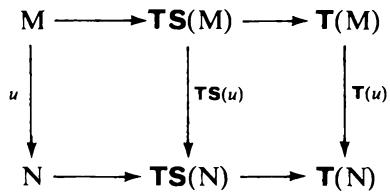
\includegraphics[keepaspectratio]{images/part001_53632150.jpg}}

是交换的，其中水平箭头表示典范单射。

若 M 是 N 的一个直因子，且 \(i: M \rightarrow N\) 是典范单射，则 \(\mathbf{TS}(i)\) 是从 \(\mathbf{TS}(\mathbf{M})\) 到 \(\mathbf{TS}(\mathbf{N})\) 的一个直因子 R 上的单同态，我们通常借此把 \(\mathbf{TS}(\mathbf{M})\) 与 R 等同。其证明与张量代数的证明相同（III，第 487 页）。

假设 M 是一个子模族 \((\mathbf{M}_{\lambda})_{\lambda \in L}\) 的直和。典范单射 \(\mathbf{TS}(\mathbf{M}_{\lambda}) \to \mathbf{TS}(\mathbf{M})\) 定义了分次代数的一个保单位同态 h，称为典范同态：

\[
\underset {\lambda \in L} {\otimes} \mathbf {T S} \left(\mathrm{M} _ {\lambda}\right)\rightarrow \mathbf {T S} (\mathrm{M}).
\]

设 \(\lambda_1, \lambda_2, \ldots, \lambda_n\) 是 \(L\) 中两两不同的元素，并令 \(x_1 \in M_{\lambda_1}, \ldots, x_n \in M_{\lambda_n}\) 。根据 IV 第 45 页命题 3 (ii)，我们有

\[
h \left(\sum_ {p _ {1} + \dots + p _ {n} = p} \gamma_ {p _ {1}} (x _ {1}) \otimes \dots \otimes \gamma_ {p _ {n}} (x _ {n})\right) = \gamma_ {p} (x _ {1} + \dots + x _ {n}).\tag{8}
\]

设 N 是一个 A-模，它是子模族 \((\mathbf{N}_{\lambda})_{\lambda \in L}\) 的直和。对于每一个 \(\lambda \in L\) ，令 \(u_{\lambda}\) 是从 \(M_{\lambda}\) 到 \(N_{\lambda}\) 的一个同态。设 u 是由 \(u_{\lambda}\) 定义的从 M 到 N 的同态。则图表

\[
\begin{array}{c} \otimes \mathsf {T S} (\mathrm{M} _ {\lambda}) \xrightarrow {h} \mathsf {T S} (\mathrm{M}) \\ \otimes \mathsf {T S} (u _ {\lambda}) \Bigg | _ {\downarrow} \qquad \qquad \qquad \qquad \qquad \qquad \qquad \qquad \qquad \qquad \qquad \qquad \qquad \qquad \qquad \qquad \qquad \qquad \qquad \qquad \qquad \qquad \qquad \qquad \qquad \qquad \qquad \qquad \qquad \qquad \qquad \qquad \qquad \qquad \\ \otimes \mathsf {T S} (\mathrm{N} _ {\lambda}) \xrightarrow {h ^ {\prime}} \mathsf {T S} (\mathrm{N}) \end{array}
\]

可交换，其中 h 和 \(h'\) 是典范同态。因为若 \(z \in TS(M_{\lambda})\) ，且 \(i_{\lambda}\) （相应地 \(j_{\lambda}\) ）表示 \(M_{\lambda}\) 到 M 的典范单射（相应地，\(N_{\lambda}\) 到 N 的典范单射），则我们有

\[
\begin{array}{r l} \mathbf {T S} (u) (h (z)) & = \mathbf {T S} (u) \circ \mathbf {T S} (i _ {\lambda}) (z) = \mathbf {T S} (u \circ i _ {\lambda}) (z) = \\ & = \mathbf {T S} (j _ {\lambda} \circ u _ {\lambda}) (z) = \mathbf {T S} (j _ {\lambda}) \circ \mathbf {T S} (u _ {\lambda}) (z) = h ^ {\prime} (\mathbf {T S} (u _ {\lambda}) (z)). \end{array}
\]

命题 6. --- 设 M 是一个 A-模，它是子模族 \((\mathbf{M}_{\lambda})_{\lambda \in L}\) 的直和。若每个 \(M_{\lambda}\) 是自由模，则从 \(\otimes \mathbf{TS}(\mathbf{M}_{\lambda})\) 到 \(\mathbf{TS}(\mathbf{M})\) 的典范同态是一个同构。

设 \((e_{i,\lambda})_{i\in I_{\lambda}}\) 是 \(\mathbf{M}_{\lambda}\) 的一组基。对于 \(\nu \in \mathbf{N}^{(I_{\lambda})}\) ，令 \(e_{\nu ,\lambda} = \prod_{i\in I_{\lambda}}\gamma_{\nu (i)}(e_{i,\lambda})\) 。这些 \(e_{\nu ,\lambda}\) （\(\nu \in \mathbf{N}^{(I_{\lambda})}\) ）构成 \(\mathbf{TS}(\mathbf{M}_{\lambda})\) 的一组基（IV，第 47 页，命题 4 (i)），且 \(e_{0,\lambda}\) 是 \(\mathbf{TS}(\mathbf{M}_{\lambda})\) 的单位元。因此这些元素

\[
\bigotimes_ {\lambda \in L} e _ {\nu_ {\lambda}, \lambda}\tag{9}
\]

，其中 \(\nu_{\lambda} \in \mathbf{N}^{(I_{\lambda})}\) 且除有限多个指标外 \(\nu_{\lambda} = 0\) ，构成 \(\otimes_{\lambda} \mathbf{TS}(M_{\lambda})\) 的一组基。命题中的典范同态把元素 (9) 映为 \(\prod_{\lambda \in L} e_{\nu_{\lambda,\lambda}}\) 。如果我们用 \((e_i)_{i \in I}\) 表示这些族 \((e_{i,\lambda})_{i \in I_{\lambda}}\) 的不交并，则上述元素恰好是 \(\prod_{i \in I} \gamma_{\nu(i)}(e_i)\) （其中 \(\nu \in \mathbf{N}^{(I)}\) ），因此它们构成 \(\mathbf{TS}(M)\) 的一组基。这就证明了该命题。

在命题 6 的条件下，逆同构 \(\mathbf{TS}(\mathbf{M}) \to \otimes_{\lambda} \mathbf{TS}(\mathbf{M}_{\lambda})\) 也称为典范的。通常把 \(\mathbf{TS}(\mathbf{M})\) 与

\(\otimes_{\lambda} \mathbf{TS}(M_{\lambda})\) 借助此同构等同起来。应当注意，若 \(z \in \mathbf{TS}(M_{\lambda})\)

\pandocbounded{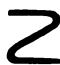
\includegraphics[keepaspectratio]{images/part001_3a9079a2.jpg}}

且 \(z' \in \mathbf{TS}(M_{\mu})\) （\(\lambda \neq \mu\) ），那么我们由此被引导用 \(z \otimes z'\) 表示的 TS(M) 的元素并不是 z 与 \(z'\) 在 T(M) 中的张量积，而是 z 与 \(z'\) 的对称积。

命题 7. --- 设 M 为一个 A-模，u 为映射 \((x, y) \mapsto x + y\) （从 \(M \oplus M\) 到 M 中），且 f 为复合映射

\[
\mathbf {T S} (\mathrm{M}) \otimes \mathbf {T S} (\mathrm{M}) \xrightarrow {h} \mathbf {T S} (\mathrm{M} \oplus \mathrm{M}) \xrightarrow {\mathbf {T S} (u)} \mathbf {T S} (\mathrm{M})
\]

，其中 \(h\) 是典范同态。若 \(z, z' \in \mathbf{TS}(\mathbf{M})\) ，则 \(f(z \otimes z') = zz'\) 。

设 \(i\) 为映射 \(x \mapsto (x, 0)\) （从 M 到 M ⊕ M 中的）。我们有 \(u \circ i = \mathrm{Id}_{\mathbf{M}}\) ，因此 \(\mathbf{TS}(u) \circ \mathbf{TS}(i) = \mathrm{Id}_{\mathbf{TS}(\mathbf{M})}\) ；因此

\[
f (z \otimes 1) = \mathbf {T S} (u) (h (z \otimes 1)) = \mathbf {T S} (u) (\mathbf {T S} (i) (z)) = z.
\]

同样地 \(f(1 \otimes z') = z'\) ，从而 \(f(z \otimes z') = f(z \otimes 1)\) \(f(1 \otimes z') = zz'\) 。

\subsection{对称张量的余积}

设 M 为自由 A-模，且 \(\Delta_{M} = \Delta\) 为对角同态 \(x \mapsto (x, x)\) （把 M 映入 \(M \oplus M\) ）。设 \(c_{M} = c\) 为由以下同态组成的分次 A-代数的保单位同态：

\[
\mathbf {T S} (\mathrm{M}) \xrightarrow {\mathbf {T S} (\Delta)} \mathbf {T S} (\mathrm{M} \oplus \mathrm{M}) \xrightarrow {\sigma} \mathbf {T S} (\mathrm{M}) \otimes \mathbf {T S} (\mathrm{M})
\]

，其中 \(\sigma\) 是典范同构。配备 \(c\) ，\(\mathbf{TS}(\mathbf{M})\) 是一个分次 A-余代数。

对所有 \(x \in \mathbf{M}\) 及每个整数 \(p \geqslant 0\) ，我们有 \(\mathbf{TS}(\Delta) (\gamma_p(x)) = \gamma_p((x, x))\) ，因此由 (8)，

\[
c \left(\gamma_ {p} (x)\right) = \sum_ {r + s = p} \gamma_ {r} (x) \otimes \gamma_ {s} (x).\tag{10}
\]

特别地

\[
c (x) = x \otimes 1 + 1 \otimes x.\tag{11}
\]

设 \((x_{i})_{i\in I}\) 是 \(\mathbf{M}\) 的一个元素族，且对于 \(\nu \in \mathbf{N}^{(I)}\) ，令 \(x_{\nu} = \prod_{i\in I}\gamma_{\nu_i}(x_i)\) 。则

\[
c \left(x _ {\nu}\right) = \sum_ {\rho + \sigma = \nu} x _ {\rho} \otimes x _ {\sigma}.\tag{12}
\]

这由(10)得出，因为 \(c\) 是一个代数同态。

命题 8. --- 设 M 是自由 A-模，则以其代数与余代数结构，TS(M) 是一个分次交换且余交换的双代数。余单位是 A-线性映射 \(\varepsilon: \mathbf{TS}(\mathbf{M}) \to \mathbf{TS}^0(\mathbf{M}) = \mathbf{A}\) ，它在 \(\mathbf{TS}^p(\mathbf{M})\) （\(p > 0\) ）上为零，且满足 \(\varepsilon(1) = 1\) 。

我们知道 A-代数 TS(M) 是结合的、交换的且含单位元的。另一方面，余积按构造是分次代数的同态；而余代数 TS(M) 是余结合且余交换的这一事实，可由公式 (10) 通过简单计算得出。映射 \(\varepsilon\) 从 TS(M) 到 A 是分次代数的同态，且满足 \(\varepsilon(1)=1\) 。最后，对每个 \(x\in M\) 我们有 \(\varepsilon(\gamma_{p}(x))=0\) ，若 p\textgreater0, \(\varepsilon(\gamma_{0}(x))=1\) ；若我们记住 (10)，这表明 \((\varepsilon\otimes1)\circ c=(1\otimes\varepsilon)\circ c=\mathrm{Id}_{\mathbf{TS}(\mathbf{M})}\) ；因此 \(\varepsilon\) 是 TS(M) 的余单位。

命题 9. --- 设 M 和 N 是自由 A-模，u 是 M 到 N 的一个 A-同态；则 TS(u) 是双代数同态。

因为我们有 \(\Delta_{\mathbf{N}} \circ u = (u, u) \circ \Delta_{\mathbf{M}}\) ，所以图表

\[
\begin{array}{c} \mathsf {T S (M)} \xrightarrow {\mathsf {T S} (\Delta_ {M})} \mathsf {T S (M \oplus M)} \xrightarrow {\sigma} \mathsf {T S (M)} \otimes \mathsf {T S (M)} \\ \mathsf {T S (u)} \Bigg | _ {\mathsf {T S (u)}} \\ \mathsf {T S (N)} \xrightarrow {\mathsf {T S} (\Delta_ {N})} \mathsf {T S (N \oplus N)} \xrightarrow {\tau} \mathsf {T S (N)} \otimes \mathsf {T S (N)}, \end{array}
\]

，其中 \(\sigma\) 和 \(\tau\) 是典范同构，该图表交换（IV，第 49 页）。因此 \(c_{\mathrm{N}} \circ \mathbf{T}\mathbf{S}(u) = (\mathbf{T}\mathbf{S}(u) \otimes \mathbf{T}\mathbf{S}(u)) \circ c_{\mathrm{M}}\) 。

命题 10. --- 设 M 是自由 A-模，则双代数 TS(M) 的本原元（III，第 602 页）恰为 M 的元素。

设 \((e_i)_{i\in I}\) 是 \(\mathbf{M}\) 的一组基，且对于 \(\nu \in \mathbf{N}^{(I)}\) ，令 \(e_{\nu} = \prod_{i\in I}\gamma_{\nu_i}(e_i)\) 。设

\(z = \sum_{\nu \in \mathbf{N}^{(I)}} \lambda_{\nu} e_{\nu}\) 为 \(\mathbf{T}\mathbf{S}(\mathbf{M})\) 的一个元素，则由 (12) 我们有

\[
c (z) = \sum_ {\nu} \lambda_ {\nu} \sum_ {\rho , \sigma \in \mathbf {N} ^ {(I)}, \rho + \sigma = \nu} e _ {\rho} \otimes e _ {\sigma} = \sum_ {\rho , \sigma} \lambda_ {\rho + \sigma} e _ {\rho} \otimes e _ {\sigma}
\]

因此

\[
c (z) - 1 \otimes z - z \otimes 1 = \sum_ {\rho \neq 0, \sigma \neq 0} \lambda_ {\rho + \sigma} e _ {\rho} \otimes e _ {\sigma} - \lambda_ {0} e _ {0} \otimes e _ {0}.
\]

因此

\[
\begin{array}{r l} z \text {   primitive   } & \Leftrightarrow \lambda_ {\rho + \sigma} = 0 \text {   when   } \rho \neq 0 \text {   and   } \sigma \neq 0 \text {   and   } \lambda_ {0} = 0 \\ & \Leftrightarrow \lambda_ {\nu} = 0 \text {   when   } | \nu | \neq 1 \\ & \Leftrightarrow z \in M. \end{array}
\]

\subsection{TS(M)与S(M)之间的关系}

M 到 TS(M) 中的典范单射以唯一方式延拓为 T(M) 到 TS(M) 中的一个代数同态（III，第 485 页，命题 1）。由 IV 第 43 页命题 2 (ii)，该同态就是对称化算子 s。由于代数 TS(M) 是交换的，因此存在（III，第 497 页）唯一的代数同态 \(\varphi_{M}\) （称为典范的），它从代数 S(M) 到代数 TS(M) 中，使得图表

\pandocbounded{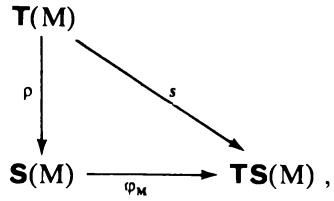
\includegraphics[keepaspectratio]{images/part001_42062a6f.jpg}}

，其中 \(\rho\) 表示 \(\mathbf{T}(\mathbf{M})\) 到 \(\mathbf{S}(\mathbf{M})\) 上的典范同态，图表交换。我们有 \(\varphi_{\mathbf{M}}(\mathbf{S}^{p}(\mathbf{M})) \subset \mathbf{T}\mathbf{S}^{p}(\mathbf{M})\) （对所有 \(p \in N\) ）。

另一方面，把 TS(M) 到 T(M) 的典范单射 i 与 T(M) 到 S(M) 的典范同态 \(\rho\) 复合，我们得到分次 A-模的一个同态 \(\psi_{M}\) ，称为典范的。图表

\pandocbounded{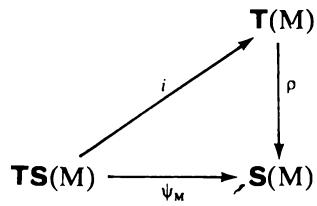
\includegraphics[keepaspectratio]{images/part001_38781a0a.jpg}}

是交换的。

如果 \(u: \mathbf{M} \to \mathbf{N}\) 是A-模的同态，则图表

\begin{enumerate}
\def\labelenumi{(\arabic{enumi})}
\setcounter{enumi}{12}
\tightlist
\item
\end{enumerate}

\pandocbounded{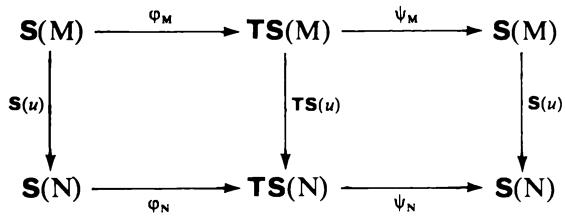
\includegraphics[keepaspectratio]{images/part001_026b2058.jpg}}

是交换的，这很容易验证。

若M是模 \(M_{\lambda}\) 的直和，则图表

\begin{enumerate}
\def\labelenumi{(\arabic{enumi})}
\setcounter{enumi}{13}
\tightlist
\item
\end{enumerate}

\pandocbounded{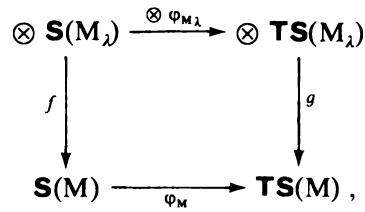
\includegraphics[keepaspectratio]{images/part001_9b5b14d2.jpg}}

，其中 \(f\) 和 \(g\) 是典范同态，是交换的。因为 \(g \circ \bigotimes_{\lambda} \varphi_{M_{\lambda}}\) 与 \(\varphi_{M} \circ f\) 都是代数同态，且它们在 \(M_{\lambda}\) 上（对每个 \(\lambda\) ）取值一致。

命题 11. --- 若 M 是自由的，则 \(\varphi_{\mathbf{M}}\) 是分次双代数的一个态射。

利用图表（13）和（14）的交换性，我们得到交换图表

\[
\begin{array}{l} \mathbf {S} (\mathrm{M}) \xrightarrow {\mathbf {S} (\Delta)} \mathbf {S} (\mathrm{M} \oplus \mathrm{M}) \xrightarrow {h} \mathbf {S} (\mathrm{M}) \otimes \mathbf {S} (\mathrm{M}) \\ \varphi_ {\mathrm{M}} \Bigg | _ {\downarrow} \quad \Bigg | _ {\varphi_ {\mathrm{M}} \oplus \mathrm{M}} \quad \Bigg | _ {\varphi_ {\mathrm{M}} \otimes \varphi_ {\mathrm{M}}} \\ \mathbf {T S} (\mathrm{M}) \xrightarrow [ \mathsf {T S} (\Delta) ]{} \mathbf {T S} (\mathrm{M} \oplus \mathrm{M}) \xrightarrow [ k ]{} \mathbf {T S} (\mathrm{M}) \cdot \otimes \mathbf {T S} (\mathrm{M}), \end{array}
\]

，其中 \(\Delta\) 是对角同态，而 h、k 是典范同态。命题由此得证。

命题 12. --- (i) 若 \(u \in \mathbf{S}^n(\mathbf{M})\) ，则 \(\psi_{\mathbf{M}}(\varphi_{\mathbf{M}}(u)) = n!u\) 。

\begin{enumerate}
\def\labelenumi{(\roman{enumi})}
\setcounter{enumi}{1}
\tightlist
\item
  若 \(v \in \mathbf{T}\mathbf{S}^n(\mathbf{M})\) ，则 \(\varphi_{\mathbf{M}}(\psi_{\mathbf{M}}(v)) = n!v\) 。
\end{enumerate}

设 \(x_{1}, \ldots, x_{n} \in M\) ，并令 u 为乘积 \(x_{1} \ldots x_{n}\) （在 \(\mathbf{S}(\mathbf{M})\) 中计算的）。则 \(\varphi_{\mathbf{M}}(u)\) 是乘积 \(x_{1} \ldots x_{n}\) （在 \(\mathbf{T}\mathbf{S}(\mathbf{M})\) 中计算的），即

\[
\sum_ {\sigma \in \mathfrak {S} _ {n}} x _ {\sigma (1)} \otimes \dots \otimes x _ {\sigma (n)}.
\]

因此 \(\psi_{\mathbf{M}}(\varphi_{\mathbf{M}}(u))\) 等于 \(\sum_{\sigma \in \mathfrak{S}_n}x_{\sigma (1)}\ldots x_{\sigma (n)}\) （在 \(\mathbf{S}(\mathbf{M})\) 中计算的），即

\[
n! x _ {1} \dots x _ {n} = n! u.
\]

设 \(v = \sum_{i=1}^{p} x_1^i \otimes x_2^i \otimes \ldots \otimes x_n^i\) 为 \(\mathbf{TS}^n(\mathbf{M})\) 的一个元素，其中 \(x_j^i\) 属于

\(\mathbf{M}\) ；则 \(\psi_{\mathbf{M}}(v)\) 等于 \(\sum_{i=1}^{p} x_1^i x_2^i \ldots x_n^i\) （在 \(\mathbf{S}(\mathbf{M})\) 中计算的），从而

\[
\varphi_ {\mathrm{M}} \big (\psi_ {\mathrm{M}} (v) \big) = \sum_ {i = 1} ^ {p} \mathbf {s} \big (x _ {1} ^ {i} \otimes x _ {2} ^ {i} \otimes \dots \otimes x _ {n} ^ {i} \big) = s (v) = n! v.
\]

推论 1. --- 若 A 是 Q-代数，则 S(M) 到 TS(M) 的典范同态是代数同构。若进一步 M 是自由的，则它是分次双代数的同构。

推论 2. --- 若 A 是一个 Q-代数，则模 \(\mathbf{TS}^n (\mathbf{M})\) 由 \(n\) 次幂（\(\mathbf{M}\) 的元素在 \(\mathbf{TS}(\mathbf{M})\) 中的）生成。

这由推论 1 及 \(\mathbf{S}(\mathbf{M})\) 的相应性质（III，第 498 页）得出。

\subsection{齐次多项式映射}

命题 13. --- 设 M 和 N 为 A-模，q 为整数 ≥ 0，f 为从 M 到 N 的一个映射。假设 M 是自由的，则下列条件等价：

\begin{enumerate}
\def\labelenumi{(\roman{enumi})}
\item
  存在一个 \(q\) -线性映射 \(g\) （从 \(\mathbf{M}^q\) 到 \(\mathbf{N}\) 中的），使得 \(f(x) = g(x, x, \ldots, x)\) （对所有 \(x \in \mathbf{M}\) ）。
\item
  存在一个线性映射 \(h\) （从 \(\mathbf{T}\mathbf{S}^q (\mathbf{M})\) 到 \(\mathbf{N}\) 中的），使得 \(f(x) = h(\gamma_q(x))\) （对所有 \(x \in \mathbf{M}\) ）。
\item
  存在一个基 \((e_i)_{i\in I}\) （\(\mathbf{M}\) 的）以及一个族 \((u_{\nu})_{\nu \in \mathbf{N}^{(I)},|\nu| = q}\) （由 \(\mathbf{N}\) 的元素组成），使得
\end{enumerate}

\[
f \left(\sum_ {i \in I} \lambda_ {i} e _ {i}\right) = \sum_ {\nu \in \mathbf {N} ^ {(I)}, | \nu | = q} \lambda^ {\nu} u _ {\nu}\tag{15}
\]

对所有 \((\lambda_i) \in \mathbf{A}^{(I)}\) 。

\begin{enumerate}
\def\labelenumi{(\roman{enumi})}
\setcounter{enumi}{3}
\tightlist
\item
  对于每个基 \((e_i)_{i\in I}\) （\(\mathbf{M}\) 的），存在一个族 \((u_{\nu})_{\nu\in \mathbf{N}^{(I)},|\nu| = q}\) （由 \(\mathbf{N}\) 的元素组成），使得
\end{enumerate}

\[
f \left(\sum_ {i \in I} \lambda_ {i} e _ {i}\right) = \sum_ {\nu \in \mathbf {N} ^ {(I)}, | \nu | = q} \lambda^ {\nu} u _ {\nu}
\]

对所有 \((\lambda_i) \in \mathbf{A}^{(\mathrm{I})}\) 。

\begin{enumerate}
\def\labelenumi{(\roman{enumi})}
\tightlist
\item
  \(\Rightarrow\) (ii)：设 \(g\) 满足 (i)，则存在一个线性映射 \(g'\) （从 \(\mathbf{T}^q (\mathbf{M})\) 到 \(\mathbf{N}\) 中的），使得 \(g(x_{1},x_{2},\ldots ,x_{q}) = g'(x_{1}\otimes x_{2}\otimes \ldots \otimes x_{q})\) （对任意 \(x_{1},\ldots ,x_{q}\in \mathbf{M}\) ）。则
\end{enumerate}

\[
f (x) = g (x, x, \dots , x) = g ^ {\prime} (x \otimes x \otimes \dots \otimes x) = g ^ {\prime} (\gamma_ {q} (x));
\]

并且写 \(h = g' \mid \mathbf{TS}^q(\mathbf{M})\) ，我们看到条件 (ii) 成立。

\begin{enumerate}
\def\labelenumi{(\roman{enumi})}
\setcounter{enumi}{1}
\tightlist
\item
  \(\Rightarrow\) (i) 和 (iv)：令 \(h\) 满足 (ii) 的条件。根据命题 4 (ii)（IV，第 47 页），存在一个线性映射 \(g'\) （从 \(\mathbf{T}^q (\mathbf{M})\) 到 \(\mathbf{N}\) 中的），使得 \(h = g'|\mathbf{TS}^q (\mathbf{M})\) 。设 \(g\) 为 \(q\) -线性映射（从 \(\mathbf{M}\) 到 \(\mathbf{N}\) 中的、与 \(g'\) 相关联的），那么对任意 \(x\in \mathbf{M}\) 我们有
\end{enumerate}

\[
f (x) = h \left(\gamma_ {q} (x)\right) = g ^ {\prime} (x \otimes x \otimes \dots \otimes x) = g (x, x, \dots , x),
\]

由此得 (i)。另一方面，若 \((e_i)_{i\in I}\) 是 \(\mathbf{M}\) 的一组基，则由公式 (6)（IV，第 46 页）有

\[
f \left(\sum_ {i} \lambda_ {i} e _ {i}\right) = h \left(\gamma_ {q} \left(\sum_ {i} \lambda_ {i} e _ {i}\right)\right) = h \left(\sum_ {| \nu | = q} \lambda^ {\nu} e _ {\nu}\right)
\]

其中记 \(e_{\nu} = \prod_{i\in I}\gamma_{\nu_i}(e_i)\) ；于是我们得到

\[
f \left(\sum_ {i} \lambda_ {i} e _ {i}\right) = \sum_ {| \nu | = q} \lambda^ {\nu} h \left(e _ {\nu}\right).
\]

\begin{enumerate}
\def\labelenumi{(\roman{enumi})}
\setcounter{enumi}{3}
\item
  \(\Rightarrow\) (iii) 是显然的。
\item
  \(\Rightarrow\) (ii)：给定满足 (iii) 条件的 \((e_i)\) 与 \((u_\nu)\) ，令 \(e_\nu = \prod_{i\in I}\gamma_{\nu_i}(e_i)\) ，并回想 \((e_\nu)_{|\nu| = q}\) 是 \(\mathbf{TS}^q (\mathbf{M})\) 的一组基。设 \(h\) 为从 \(\mathbf{TS}^q (\mathbf{M})\) 到 \(\mathbf{N}\) 中的、由 \(h(e_{\nu}) = u_{\nu}\) 定义的同态；则对每个 \(x = \sum_{i\in I}\lambda_i e_i\) （\(\mathbf{M}\) 中的）我们有
\end{enumerate}

\[
f (x) = f \left(\sum_ {i} \lambda_ {i} e _ {i}\right) = \sum_ {| \nu | = q} \lambda^ {\nu} u _ {\nu} = h \left(\sum_ {| \nu | = q} \lambda^ {\nu} e _ {\nu}\right) = h (\gamma_ {q} (x)).
\]

定义 3. --- 设 M 和 N 为 A-模，q 为整数 \(\geqslant 0\) 。假设 M 是自由的，并用 \(\operatorname{Pol}_{\mathbf{A}}^{q}(\mathbf{M}, \mathbf{N})\) 或简记作 \(\operatorname{Pol}^{q}(\mathbf{M}, \mathbf{N})\) 表示满足命题 13 各条件的从 M 到 N 的映射组成的集合。\(\operatorname{Pol}^{q}(\mathbf{M}, \mathbf{N})\) 的元素称为从 M 到 N 的 q 次齐次多项式映射。

命题 13 (i) 定义了一个 A-模同态：

\[
\mathcal {L} _ {q} (\mathrm{M}, \dots , \mathrm{M}; \mathrm{N}) \rightarrow \operatorname{Pol} ^ {q} (\mathrm{M}, \mathrm{N}).
\]

命题 13 (ii) 定义了一个 A-模同态：

\[
\operatorname{Hom} _ {\mathrm{A}} \left(\mathbf {T S} ^ {q} (\mathrm{M}), \mathrm{N}\right)\rightarrow \operatorname{Pol} ^ {q} (\mathrm{M}, \mathrm{N}).
\]

这些同态称为典范同态。它们是满射的。

例子. --- 1) 从 M 到 N 的 1 次齐次多项式映射就是 M 到 N 的 A-线性映射。

\begin{enumerate}
\def\labelenumi{\arabic{enumi})}
\setcounter{enumi}{1}
\tightlist
\item
  设 \((\mathbf{N}_i)_{i\in I}\) 是一族 A-模，\(f_{i}\) 是从 \(\mathbf{M}\) 到 \(\mathbf{N}_i\) 中的映射（\(i\in I\) ），且 \(f:\mathbf{M}\to \prod_{i\in I}\mathbf{N}_i\) 为以 \(f_{i}\) 为分量的映射。为使 \(f\) 为
\end{enumerate}

q 次齐次多项式映射，必要且充分条件是每个 \(f_{i}\) 都是 q 次齐次多项式映射。

\begin{enumerate}
\def\labelenumi{\arabic{enumi})}
\setcounter{enumi}{2}
\item
  设 \((\mathbf{M}_j)_{j\in J}\) 是自由 A-模的一个有限族，且 \(u:\prod_{j\in J}\mathbf{M}_j\to \mathbf{N}\) 是一个多重线性映射；则 \(u\) 是次数为 Card(J) 的多项式映射。
\item
  设 \((\mathbf{X}_i)_{i\in I}\) 是未定元族，N 是一个 A-模，且 \(u\in \mathbf{N}[(\mathbf{X}_i)_{i\in I}]\) 是次数为 \(q\) 的齐次多项式。映射 \((x_{i})_{i\in I}\mapsto u((x_{i})_{i\in I})\) （\(\mathbf{A}^{(I)}\) 到 N 中的）是次数为 \(q\) 的齐次多项式映射：这由命题 13 的条件 (iii) 立即可见。若 I 有限，则每个次数为 \(q\) 的、从 \(\mathbf{A}^{(I)} = \mathbf{A}^{\mathrm{I}}\) 到 N 的齐次多项式映射都具有该形式。
\item
  映射 \((x_{i})_{i\in\mathbf{N}}\mapsto x_{0}^{2}+x_{1}^{2}+\cdots+x_{n}^{2}+\cdots\) （\(\mathbf{A}^{(N)}\) 到 A 中的）是次数为 2 的齐次多项式映射。若 A=Z/2Z，则它与线性映射 \((x_{i})_{i\in I}\mapsto x_{0}+x_{1}+\cdots+x_{n}+\cdots\)
\item
  设 \(f \in \operatorname{Pol}_{\mathbf{A}}^{q}(\mathbf{M}, \mathbf{N})\) ，设 \(\mathbf{B}\) 是一个交换环，\(\rho\) 是从 \(\mathbf{B}\) 到 \(\mathbf{A}\) 中的一个同态，而 \(\mathbf{M}'\) 与 \(\mathbf{N}'\) 是由 \(\mathbf{M}\) 与 \(\mathbf{N}\) 通过 \(\rho\) 得到的 B-模。假设 \(\mathbf{M}'\) 是自由的；则 \(f \in \operatorname{Pol}_{\mathbf{B}}^{q}(\mathbf{M}', \mathbf{N}')\) ：这由命题 13 的条件 (i) 立即得出。
\end{enumerate}

命题 14. --- 设 M、N、P 为 A-模，q 和 r 为整数 ≥ 0，并假设 M 和 N 是自由的。若 \(f \in \text{Pol}^{q}(M, N)\) ，\(f' \in \text{Pol}^{r}(N, P)\) ，则 \(f' \circ f \in \text{Pol}^{qr}(M, P)\) 。

存在一个从 \(M^{q}\) 到 N 中的 q-线性映射 g，以及一个 r-线性映射 \(g'\) （从 \(N^{r}\) 到 P 中的），使得

\[
\begin{array}{l l} f (x) = g (x, x, \dots , x) & \text { for   all } x \in \mathbf {M}, \\ f ^ {\prime} (y) = g ^ {\prime} (y, y, \dots , y) & \text { for   all } y \in \mathbf {N}. \end{array}
\]

因此对每个 \(x \in \mathbf{M}\) 我们有

\[
f ^ {\prime} (f (x)) = g ^ {\prime} (f (x), f (x), \dots , f (x)) = g ^ {\prime} (g (x, x, \dots , x), \dots , g (x, x, \dots , x))
\]

且映射 \((x_{1},\ldots ,x_{qr})\mapsto g^{\prime}\big(g(x_{1},\dots,x_{q}),\dots,g(x_{q(r - 1) + 1},\dots,x_{qr})\big)\) （\(\mathbf{M}^{qr}\) 到 \(\mathbf{P}\) 中的）是 \(qr\) -线性的。

命题 15. --- 设 M 为自由 A-模，N 为 A-模，q 为整数 \(\geqslant0\) 。我们假设映射 \(y\mapsto q!y\) 是 N 的一个自同构。设 \(f\in\mathrm{Pol}^{q}(\mathbf{M},\mathbf{N})\) ，则存在唯一的、从 \(M^{q}\) 到 N 的对称 q-线性映射 h，使得 \(f(x)=h(x,x,\ldots,x)\) （对所有 \(x\in M\) ）。对任意 \(x_{1},\ldots,x_{q}\in M\) 我们有

\[
h \left(x _ {1}, x _ {2}, \dots , x _ {q}\right) = \frac {(- 1) ^ {q}}{q !} \sum_ {\mathrm{H} \subset \{1, 2, \dots , q \}} (- 1) ^ {\text { Card   H }} f \left(\sum_ {i \in \mathrm{H}} x _ {i}\right).\tag{16}
\]

\begin{enumerate}
\def\labelenumi{\alph{enumi})}
\tightlist
\item
  存在一个 \(q\) -线性映射 \(g\) （从 \(\mathbf{M}^q\) 到 \(\mathbf{N}\) 中的），使得 \(f(x) = g(x, x, \ldots, x)\) （对所有 \(x \in \mathbf{M}\) ）。我们定义一个 \(q\) -线性映射 \(h\) （从 \(\mathbf{M}\) 到 \(\mathbf{N}\) 中的），由
\end{enumerate}

\[
h \left(x _ {1}, x _ {2}, \dots , x _ {q}\right) = \frac {1}{q !} \sum_ {\sigma \in \mathfrak {S} _ {q}} g \left(x _ {\sigma (1)}, x _ {\sigma (2)}, \dots , x _ {\sigma (q)}\right).
\]

则 \(h\) 是对称的，且 \(f(x) = h(x, x, \ldots, x)\) （对所有 \(x \in \mathbf{M}\) ）。

\begin{enumerate}
\def\labelenumi{\alph{enumi})}
\setcounter{enumi}{1}
\tightlist
\item
  设 \(h\) 为对称的 \(q\) -线性映射（从 \(\mathbf{M}^q\) 到 \(\mathbf{N}\) 中的），使得 \(f(x) = g(x, x, \ldots, x)\) 。设 \(l\) 为线性映射（从 \(\mathbf{T}^q(\mathbf{M})\) 到 \(\mathbf{N}\) 中的），使得 \(h(x_1, \ldots, x_q) = l(x_1 \otimes \ldots \otimes x_q)\) （对任意 \(x_1, \ldots, x_q \in \mathbf{M}\) ）。我们有
\end{enumerate}

\[
\begin{array}{l} (- 1) ^ {q} q! h (x _ {1}, \dots , x _ {q}) = (- 1) ^ {q} \sum_ {\sigma \in \mathfrak {S} _ {q}} h (x _ {\sigma (1)}, \dots , x _ {\sigma (q)}) = \\ = (- 1) ^ {q} l (\mathbf {s} (x _ {1} \otimes \dots \otimes x _ {q})) = \sum_ {\mathrm{H} \subset \{1, \dots , q \}} (- 1) ^ {\text {Card H}} l \left(\gamma_ {q} \left(\sum_ {i \in \mathrm{H}} x _ {i}\right)\right) \end{array}
\]

这由 IV 第 45 页命题 3 (v) 得出。现在

\[
l \left(\gamma_ {q} \left(\sum_ {i \in H} x _ {i}\right)\right) = h \left(\sum_ {i \in H} x _ {i}, \dots , \sum_ {i \in H} x _ {i}\right) = f \left(\sum_ {i \in H} x _ {i}\right)
\]

这就证明了公式 (16) 及 h 的唯一性。

命题 16. --- 设 M 为自由 A-模，N 为 A-模，q 为正整数，u 为从 Hom(TS \(^{q}\) (M), N) 到 Pol \(^{q}\) (M, N) 的典范同态。

\begin{enumerate}
\def\labelenumi{(\roman{enumi})}
\item
  若 \(\mathbf{A}\) 是无限整环且 \(\mathbf{N}\) 是无挠的，则 \(u\) 是同构。
\item
  若映射 \(y \mapsto q!y\) 在 \(\mathbf{N}\) 中是单射，则 \(u\) 是同构。
\end{enumerate}

在命题的两种情形中，我们须证 \(u\) 是单射的，即每个线性映射 \(f\) （从 \(\mathbf{TS}^q(\mathbf{M})\) 到 \(\mathbf{N}\) 中的、在 \(\gamma_q(\mathbf{M})\) 上为零的）都恒为零。

假设 A 是无限整环且 N 无挠。对每个 \(z \in \mathbf{TS}^{q}(\mathbf{M})\) ，存在 \(\alpha \in A - \{0\}\) 使得 \(\alpha z\) 是 \(\gamma_{q}(\mathbf{M})\) 的元素的 A-线性组合（IV，第 47 页，命题 5）。因此 \(\alpha f(z) = f(\alpha z) = 0\) ，于是 \(f(z) = 0\) 。

其次假设映射 \(y \mapsto q!y\) 在 \(\mathbf{N}\) 中是单射的，则由 IV 第 45 页命题 3 (v)，\(f\) 在 \(\mathbf{s} \cdot \mathbf{T}^q(\mathbf{M})\) 上为零。因此若 \(z \in \mathbf{T}\mathbf{S}^q(\mathbf{M})\) ，我们有 \(q!f(z) = f(\mathbf{s}z) = 0\) ，于是 \(f(z) = 0\) 。

推论. --- 设 M 是自由 A-模，N 是 A-模，q 是正整数，\(h \in \operatorname{Pol}^{q}(M, N)\) ，且 \((e_{i})_{i \in I}\) 是 M 的一组基。在命题 16 的两种情形下，存在唯一的族 \((u_{\nu})_{\nu \in \mathbf{N}^{(I)}, |\nu| = q}\) （由 N 的元素组成），使得 \(h\left(\sum_{i \in I} \lambda_{i} e_{i}\right) = \sum_{|\nu| = q} \lambda^{\nu} u_{\nu}\) （对所有 \((\lambda_{i}) \in \mathbf{A}^{(I)}\) ）。

\subsection{多项式映射}

定义 4. --- 设 M 和 N 为 A-模，并假设 M 是自由的。设 \(\operatorname{Map}(M, N)\) 为从 M 到 N 的所有映射组成的 A-模。子模 \(\sum_{q > 0} \operatorname{Pol}_{A}^{q}(M, N)\) （\(\operatorname{Map}(M, N)\) 的）用 \(\operatorname{Pol}_{A}(M, N)\) 或简记作 \(\operatorname{Pol}(M, N)\) 表示；

其元素称为从 M 到 N 的多项式映射。

设 \((e_{i})_{i\in I}\) 是 M 的一组基，并假设 I 是有限的；由命题 13（IV，第 54 页），从 M 到 N 的映射 f 是多项式的当且仅当存在一个关于未定元 \(X_{i}\) 的、系数在 N 中的多项式 F，使得

\[
f \left(\sum_ {i \in I} x _ {i} e _ {i}\right) = F (\mathbf {x})
\]

对每个族 \(\mathbf{x} = (x_i)_{i\in I}\) （\(\mathbf{A}^{(I)}\) 中的）。该性质与为 \(\mathbf{M}\) 所选取的基无关，并且它证明了“多项式映射”这一术语的合理性。

命题 17. --- 设 M 为自由 A-模，B 为结合、交换且含单位的 A-代数。则 \(\operatorname{Pol}_{\mathbf{A}}(\mathbf{M}, \mathbf{B})\) 是代数 \(\operatorname{Map}(\mathbf{M}, \mathbf{B})\) 的一个子 B-代数。

这由定义 4 及命题 13 (iv)（IV，第 54 页）得出。

命题 18. --- 设 M、N、P 为 A-模，并假设 M 和 N 是自由的。若 \(f \in \operatorname{Pol}(M, N)\) ，\(g \in \operatorname{Pol}(N, P)\) ，则 \(g \circ f \in \operatorname{Pol}(M, P)\) 。

我们可以立即化简到存在整数 q 使得 \(g \in \text{Pol}^{q}(N, P)\) 的情形；则存在一个从 \(N^{q}\) 到 P 的 q-线性映射 h，使得 \(g(y) = h(y, y, \ldots, y)\) （对所有 \(y \in N\) ）。把 f 写成齐次多项式映射之和，我们便归结为证明映射

\[
x \mapsto h (f _ {1} (x), f _ {2} (x), \dots , f _ {q} (x))
\]

（从 M 到 P 中的），其中 \(f_{i} \in \operatorname{Pol}^{q_{i}}(\mathbf{M}, \mathbf{N})\) ，是多项式的。对 \(i = 1, \ldots, q\) ，存在一个 \(q_{i}\) -线性映射 \(l_{i}\) （从 \(M^{q_{i}}\) 到 N 中的），使得 \(f_{i}(x) = l_{i}(x, x, \ldots, x)\) （对所有 \(x \in M\) ）。因此

\[
h \left(f _ {1} (x), f _ {2} (x), \dots , f _ {q} (x)\right) = h \left(l _ {1} (x, \dots , x), \dots , l _ {q} (x, \dots , x)\right),
\]

由此，我们的论断得证。

引理2. --- 设 N 是一个 A-模，n 是一个整数 ≥0，且

\[
f = m _ {0} + m _ {1} \mathrm{X} + \dots + m _ {n} \mathrm{X} ^ {n} \in \mathrm{N} [ \mathrm{X} ].
\]

假设存在 \(\alpha_{0}, \alpha_{1}, \ldots, \alpha_{n} \in A\) 使得 \(f(\alpha_{0}) = \cdots = f(\alpha_{n}) = 0\) ，并且使得对 \(i \neq j\) ，N 中比率为 \(\alpha_{i} - \alpha_{j}\) 的位似是单射，则 f = 0。

（此引理推广了 IV 第 16 页的推论。）

引理对 \(n = 0\) 显然成立；我们将对 \(n\) 作归纳来证明它。我们有

\[
f (\mathbf {X}) = f (\mathbf {X}) - f \left(\alpha_ {0}\right) = \sum_ {i = 1} ^ {n} m _ {i} \left(\mathbf {X} ^ {i} - \alpha_ {0} ^ {i}\right) = \left(\mathbf {X} - \alpha_ {0}\right) g (\mathbf {X})
\]

其中 g 是 N{[}X{]} 的一个形如 \(m_{0}^{\prime} + m_{1}^{\prime} X + \cdots + m_{n-1}^{\prime} X^{n-1}\) 的元素。引理的假设蕴含 \(g(\alpha_{1}) = \cdots = g(\alpha_{n}) = 0\) ，因此由归纳假设得 g = 0，从而 f = 0。

命题 19. --- 设 M 为自由 A-模，N 为 A-模，G 为 A 的一个无限加法子群，并假设由 G 的非零元素定义的 N 的位似都是单射。则 \(\operatorname{Pol}(M,N)\) 是诸 \(\operatorname{Pol}^{q}(M,N)\) 的直和。

设 \(f_{0}, f_{1}, \ldots, f_{n}\) 满足 \(f_{i} \in \operatorname{Pol}^{i}(\mathbf{M}, \mathbf{N})\) ，并且假设有关系 \(f_{0} + \cdots + f_{n} = 0\) 。设 \(x \in \mathbf{M}\) ，则对所有 \(\lambda \in G\) 我们有

\[
0 = \sum_ {i = 0} ^ {n} f _ {i} (\lambda x) = \sum_ {i = 0} ^ {n} \lambda^ {i} f _ {i} (x).
\]

根据引理 2 应用于多项式 \(\sum_{i=0}^{n} f_i(x) X^i\) ，我们有

\[
f _ {0} (x) = \dots = f _ {n} (x) = 0.
\]

推论. --- 假设 A 是一个无限整环；设 M 是一个自由 A-模，N 是一个无挠 A-模。

\begin{enumerate}
\def\labelenumi{(\roman{enumi})}
\tightlist
\item
  我们有 \(\operatorname{Pol}(\mathbf{M},\mathbf{N}) = \bigoplus_{q\geqslant 0}\operatorname{Pol}^q (\mathbf{M},\mathbf{N})\) 且每个 \(\operatorname{Pol}^q (\mathbf{M},\mathbf{N})\) 可以
\end{enumerate}

典范地等同于 \(\operatorname{Hom}(\mathbf{TS}^q(\mathbf{M}),\mathbf{N})\) 。

\begin{enumerate}
\def\labelenumi{(\roman{enumi})}
\setcounter{enumi}{1}
\tightlist
\item
  设 \(f \in \operatorname{Pol}(M, N)\) ，且 \((e_i)_{i \in I}\) 是 \(M\) 的一组基。存在唯一的族 \((u_\nu)_{\nu \in \mathbb{N}^{(I)}}\) （由 \(N\) 的元素组成），使得 \(f\left(\sum_{i \in I} \lambda_i e_i\right) = \sum_{\nu \in \mathbb{N}^{(I)}} \lambda^\nu u_\nu\) （对所有
\end{enumerate}

\[
\left(\lambda_ {i}\right) \in \mathbf {A} ^ {(I)}
\]

成立。断言 (i) 由命题 16 和 19 得出，(ii) 由 (i) 及命题 16 的推论得出。
